\documentclass[letterpaper,11pt]{report}

\usepackage{fullpage}
\usepackage{verbatim}
\usepackage{cite}
\usepackage{setspace}
\usepackage{fancyhdr}
\usepackage{graphicx}
\usepackage{subcaption}
\usepackage{float}

%\usepackage{noReferences}

\usepackage{graphics}
\usepackage{color}
\documentclass{article}

\usepackage{caption}
\usepackage{amsmath}
\usepackage{geometry}
\usepackage{enumitem}
\usepackage{hyperref}

\geometry{a4paper, margin=1in}
\usepackage{hyperref}

%\usepackage{natbib}



% Paper conservation layout. Long live the trees!!
\setlength{\oddsidemargin}{-0.4mm} % 25 mm left margin
\setlength{\evensidemargin}{\oddsidemargin}
\setlength{\textwidth}{160mm}      % 25 mm right margin
\setlength{\topmargin}{-5.4mm}     % 20 mm top margin
\setlength{\headheight}{5mm}
\setlength{\headsep}{5mm}
\setlength{\footskip}{10mm}
\setlength{\textheight}{237mm}     % 20 mm bottom margin


\setlength{\parskip}{1ex}
\parindent 0in
\def\SAONE{Specific Aim 1}
\def\SATWO{Specific Aim 2}
\def\SATHREE{Specific Aim 3}
\def\SAFOUR{Specific Aim 4}

\def\title{Mytitle}
%\def\titletwo{Thesis Proposal Title Line 2}

\begin{document}

\include{btech_thesis_cover}

\newpage
\begin{titlepage}
    \centering
    \vspace*{3cm} % Adjust vertical spacing
    {\Huge\bfseries Pixel to Plate \par} % Title in bold and large font
    \vspace{3cm} % Space between title and names
    
    \large
    \textbf{Student Name:} Ieshaan Awasthy \\
    \textbf{Roll Number:} 2021054 \\[1cm]
    \textbf{Student Name:} Gunjan Dabas \\
    \textbf{Roll Number:} 2021253 \\[2cm]
    
\textit{BTP report submitted in partial fulfillment of the requirements \\ 
for the Degree of B.Tech. in Computer Science \& Engineering (Ieshaan) \\ 
and Computer Science and Applied Mathematics (Gunjan)} \\[0.5cm]

    \textbf{Date:} 5th May 2025 \\[1cm]
    \textbf{BTP Track:} Engineering Track \\[0.5cm]
    \textbf{BTP Advisor:} Dr. Ganesh Bagler \\
    
    \vfill % Push the following text to the bottom
    
    \textbf{Indraprastha Institute of Information Technology} \\
    \textbf{New Delhi}
\end{titlepage}





\begin{center}
\textbf{\Large Student's Declaration}\label{section:declaration}
\end{center}
%\vspace{3in}
I hereby declare that the work presented in the report entitled \textbf{``Pixel To Plate"} submitted by me for the partial fulfillment of the requirements for the degree of \emph{Bachelor of Technology} in \emph{Computer Science \& Engineering (Ieshaan)} and \emph{Computer Science and Applied Mathematics (Gunjan)} at
 Indraprastha Institute of Information Technology, Delhi, is an authentic record of my work carried out under guidance of \textbf{Dr.Ganesh Bagler}. Due acknowledgements have  been given in the report to all material used. This work has not been submitted anywhere else for the reward of any other degree.
 \\ \vspace{0.5in}

\textbf{Ieshaan Awasthy and Gunjan Dabas}\hfill
\textbf{ Place \& Date: 1/05/2024} \\
\textbf{(student's name)}

%\doublespacing



\vspace{3in}
%\iffalse
\begin{center}
\textbf{\Large Certificate} \label{section:certificate}
\end{center}
%\vspace{3in}
This is to certify that the above statement made by the candidate is correct to the best of my knowledge.
 \\ \vspace{0.4in}

\textbf{Dr.Ganesh Bagler}\hfill
\textbf{ Place \& Date: .............................} \\
\textbf{(advisors' name)}\\



\pagebreak

\begin{abstract}
This project, \textit{Pixel to Plate}, presents an end-to-end system that bridges computer vision and natural language processing to automate personalized recipe generation from images of ingredients. The first phase focuses on object detection, where YOLOv8x was fine-tuned on the AI-Cook dataset after comprehensive exploratory data analysis (EDA) addressing dataset quality, class imbalance, and object co-occurrence. YOLOv8x achieved a precision of 0.970, making it the selected model for robust ingredient identification.

The second phase evaluates four large language models—LLaMA, Falcon, GEMMA, and Phi—for zero-shot recipe generation based on the detected ingredients. Among them, LLaMA 3.1 produced the most coherent and contextually appropriate recipes. Prompt tuning was employed to improve generation quality and reduce inference overhead, achieving a balance between performance and efficiency.

To support real-world utility, the system incorporates agentic behavior that dynamically adapts recipes to user-specific constraints such as available ingredients, dietary restrictions, and preparation time. This context-aware generation enhances usability and personalization. Future directions include integrating quantity estimation, nutritional analysis, and deployment on interactive platforms.

This interdisciplinary project demonstrates the effectiveness of integrating cutting-edge object detection with prompt-tuned language models for intelligent culinary applications.

\vspace{2em}
\noindent\textbf{Keywords:} Object Detection, YOLOv8, Recipe Generation, Prompt Tuning, Large Language Models, AI-Cook Dataset, Natural Language Processing, Computer Vision, Culinary Applications
\end{abstract}





\section*{Acknowledgments}\label{section:acknowledgments}
\pagestyle{plain}
We would like to express our deepest gratitude to our BTP advisor, Dr. Ganesh Baglar, for his invaluable guidance, support, and encouragement throughout the duration of this project. His expertise and insightful feedback were instrumental in shaping our approach and helping us achieve our goals.

We are also extremely thankful to PhD Mansi Goel for her continuous support and encouragement, particularly in the areas of computer vision and natural language processing. Her knowledge and insights were crucial in refining our model designs and understanding the technical intricacies of this project.

Additionally, we would like to thank Madhavi Ma'am for her support and guidance throughout the project, helping us overcome challenges and ensuring we stayed on track towards completing this BTP successfully.

Finally, we extend our appreciation to the entire faculty of the Computer Science and Engineering Department at Indraprastha Institute of Information Technology, Delhi, for their constant support, encouragement, and academic resources throughout this research endeavor.

\vspace{2in}
\subsection*{Work Distribution}

The work distribution between us was equal, with both contributors equally involved in all aspects of the project. Both Ieshaan Awasthy and Gunjan Dabas contributed to the object detection phase, model evaluation, and analysis of the results. The recipe generation phase was also a collaborative effort, with both working on the evaluation of different large language models and their performance metrics.

\noindent We would like to extend our gratitude to the entire faculty and staff of the Indraprastha Institute of Information Technology, New Delhi, for their support and encouragement.
\newpage

\tableofcontents

%\newpage

%\newpage

% \newpage
\mbox{}


%\doublespacing

\chapter{Introduction}\label{chapter:introduction}
%\pagestyle{fancy}
\section{Motivation}

The motivation for this project stems from the need to integrate distinct AI capabilities, such as image recognition and natural language generation, to solve real-world problems. While advancements in these areas have been significant, their combined potential for creating practical, user-centric solutions remains underutilized. This project addresses this gap by tackling a common problem: generating recipes from the ingredients available in a refrigerator.

Determining what to cook often requires creativity, dietary considerations, and careful planning. Automating this task simplifies meal preparation, making it more efficient and accessible. By generating personalized, context-aware recipes, the system enhances convenience while addressing individual preferences such as dietary restrictions, cost, and preparation time. 

The project’s modular design is another key motivation. Unlike monolithic systems, a modular approach enables independent optimization and scalability. Each component evolves independently, allowing seamless integration of improvements in object detection or language generation technologies. This flexibility ensures adaptability and long-term relevance.

Beyond its immediate application, the project demonstrates how AI can be tailored to niche domains, offering a blueprint for similar efforts in areas like healthcare or education. By integrating vision and language capabilities, this work sets a precedent for creating intelligent systems that enhance daily life.
\section{Problem Statement}

Households often need help deciding what to cook using available ingredients, requiring effort to balance dietary restrictions, budgets, and preparation time. Existing tools lack adaptability and fail to provide personalized solutions. The challenge is to create a system that identifies ingredients from images and generates context-aware recipes. This requires integrating advanced object detection with language generation in a modular, scalable framework to deliver practical and user-centric solutions.

\chapter{Research on Existing Work}\label{chapter:Research on Existing Work}
The AI community has adopted multisensory or multimodal techniques to enhance the current generation of AI models, with the aim of achieving more comprehensive intelligent understanding. Integrating language and imagery is a well-established approach for tasks such as image captioning or generating visuals from descriptions. The Multimodal And Modular Ai Chef: Complex Recipe Generation From Imagery, addresses a growing need in AI applications to combine multimodal capabilities—specifically image recognition and language generation—to solve practical problems. The authors propose a modular framework, which effectively separates the tasks of object detection and recipe generation. Using YOLOv5 for object detection and OpenAI's GPT-3.5 for recipe generation, the system demonstrates how combining specialized models can outperform monolithic multimodal approaches in specific use cases.

\section{Introduction}
\begin{itemize}
    \item Multimodal learning, which integrates sensory inputs like text and imagery, has become a cornerstone of AI development.
    \item Existing models like CLIP, GATO, and LAION-5b exhibit capabilities in image-to-text tasks but lack coherence in maintaining context for complex applications like recipe generation.
    \item The study explores a modular alternative where image detection models identify objects and pass them to a Large Language Model (LLM) for text generation.
    \item The main goal is to create recipes tailored to constraints such as dietary restrictions, preparation time, cost, and portion sizes.
\end{itemize}

\section{Methodology}
\subsection{1. Image Detection}
\begin{itemize}
    \item Utilized YOLOv5 (small) as the object detection model, trained on the \textit{ai-cook-lcv4d} dataset, which includes 3,050 images of 30 common refrigerator items.
    \item Training involved a split of 2,896 images for training, 103 for validation, and 51 for testing.
    \item Pre-processing included augmentations such as rotation, exposure adjustments, and noise addition.
    \item Achieved a mean average precision (mAP) of 95.2\% and high recall rates for ingredient detection.
\end{itemize}

\subsection{2. Recipe Generation}
\begin{itemize}
    \item Used OpenAI's GPT-4 model for text generation.
    \item The input was a delimited list of detected ingredients, and the output included:
          \begin{itemize}
              \item Recipe title.
              \item Ingredients list with quantities.
              \item Cooking instructions with step-by-step details.
              \item Approximate preparation and cooking times.
          \end{itemize}
    \item Recipes adhered strictly to the provided ingredient list without external supplementation.
    \item Variants were generated for specific constraints such as vegan, keto, or lactose-intolerant diets.
\end{itemize}

\subsection{3. Modular API Pipeline}
\begin{itemize}
    \item The modular approach separates the image detection and text generation stages, enabling independent updates to each component.
    \item This design reduces computational overhead and allows rapid adaptation to evolving models.
    \item The system can handle scenarios like ingredient expiration tracking, meal planning, and waste reduction.
\end{itemize}

\section{Results}
\begin{itemize}
    \item Generated a 100-page recipe book featuring recipes based on 30 primary ingredients derived from 2,000 refrigerator images.
    \item Achieved high accuracy in ingredient detection, as reflected in the multi-class confusion matrix.
    \item Demonstrated versatility in generating diverse recipe variations:
          \begin{itemize}
              \item Adjusting for dietary preferences (vegan, keto, lactose-free).
              \item Optimizing for cost-efficiency and seasonal availability.
              \item Customizing portion sizes and meal types.
          \end{itemize}
    \item Showcased the ability to refine recipes interactively based on user feedback, leveraging GPT-4's long conversational memory.
\end{itemize}

\section{Discussion}
\begin{itemize}
    \item The modular design supports practical applications by optimizing resource use and enabling real-time edge deployment.
    \item Potential future enhancements include:
          \begin{itemize}
              \item Incorporating reinforcement learning to improve recipe generation based on user feedback.
              \item Expanding to include global cuisines and advanced food pairing principles.
              \item Adding operational research capabilities for cost optimization in large-scale settings like restaurants.
          \end{itemize}
    \item Highlights the environmental benefits of reducing food waste through efficient inventory utilization.
\end{itemize}

\section{Conclusion}
The study demonstrates a scalable, practical solution for AI-based recipe generation by combining state-of-the-art image detection and language generation models. The modular API approach outperforms monolithic models in adaptability and efficiency, enabling complex human-like culinary tasks in real-world scenarios.

% \subsection*{Relevance to AI Trends}
% \begin{itemize}[noitemsep]
%     \item Aligns with leveraging large language models (LLMs) for real-world applications.
%     \item Emphasizes multimodal AI solutions for everyday needs.
% \end{itemize}

% \section*{Limitations}
% \begin{itemize}[noitemsep]
%     \item \textbf{Dataset Constraints:} The AI-Cook dataset is relatively small (30 ingredient classes), limiting generalization.
%     \item \textbf{Dependence on LLMs:} Reliance on ChatGPT raises adaptability concerns for newer models.
%     \item \textbf{Lack of Detailed User Studies:} User evaluations could assess the generated recipes' usability.
    % \item \textbf{Limited Exploration of Multimodal Fusion:} Modular design not rigorously compared to state-of-the-art multimodal systems such as CLIP or GATO.
% \end{itemize}


\chapter{Work Done}\label{chapter:Work Done}

\section{Object Detection}
The primary focus of this phase was to identify the most suitable object detection model for the AI-Cook dataset. This model will be used to detect ingredients and subsequently facilitate automated recipe generation. Below are the detailed steps and outcomes of this phase:

\subsection{Dataset Preparation}
The dataset was sourced from Roboflow and thoroughly analyzed to ensure its readiness for model training. Key aspects of the dataset are as follows:
\begin{itemize}
    \item \textbf{Structure:} The dataset consists of 3,040 images with corresponding label files, organized into training (2,896 images), validation (93 images), and test sets (51 images).
    \item \textbf{Image Properties:} All images have uniform dimensions of 640x640 pixels, ensuring consistency during training.
    \item \textbf{Class Distribution:} Class imbalance was noted, with some categories underrepresented. Frequent co-occurrence of specific class pairs (e.g., bread \& butter) provides valuable insights for future tasks.
    \item \textbf{Bounding Boxes:} Bounding box sizes varied, with most being relatively small compared to the image size. This was confirmed by analyzing the bounding box-to-image size ratio.
    \item \textbf{Object Density:} Most images contain multiple objects, which enhances the dataset's representativeness for real-world scenarios.
\end{itemize}

\subsection{Exploratory Data Analysis (EDA)}
Detailed EDA was conducted to address potential issues such as class imbalance and data quality. Highlights include:
\begin{itemize}
    \item No duplicate or blurry images were found in the dataset.
    \item Analysis of object co-occurrence and density provided insights into natural groupings of ingredients.
\end{itemize}

% \usepackage{subcaption} % Add this to your preamble

\begin{figure}[h!]
    \centering
    % First row of images
    \begin{subfigure}[t]{0.4\textwidth}
        \centering
        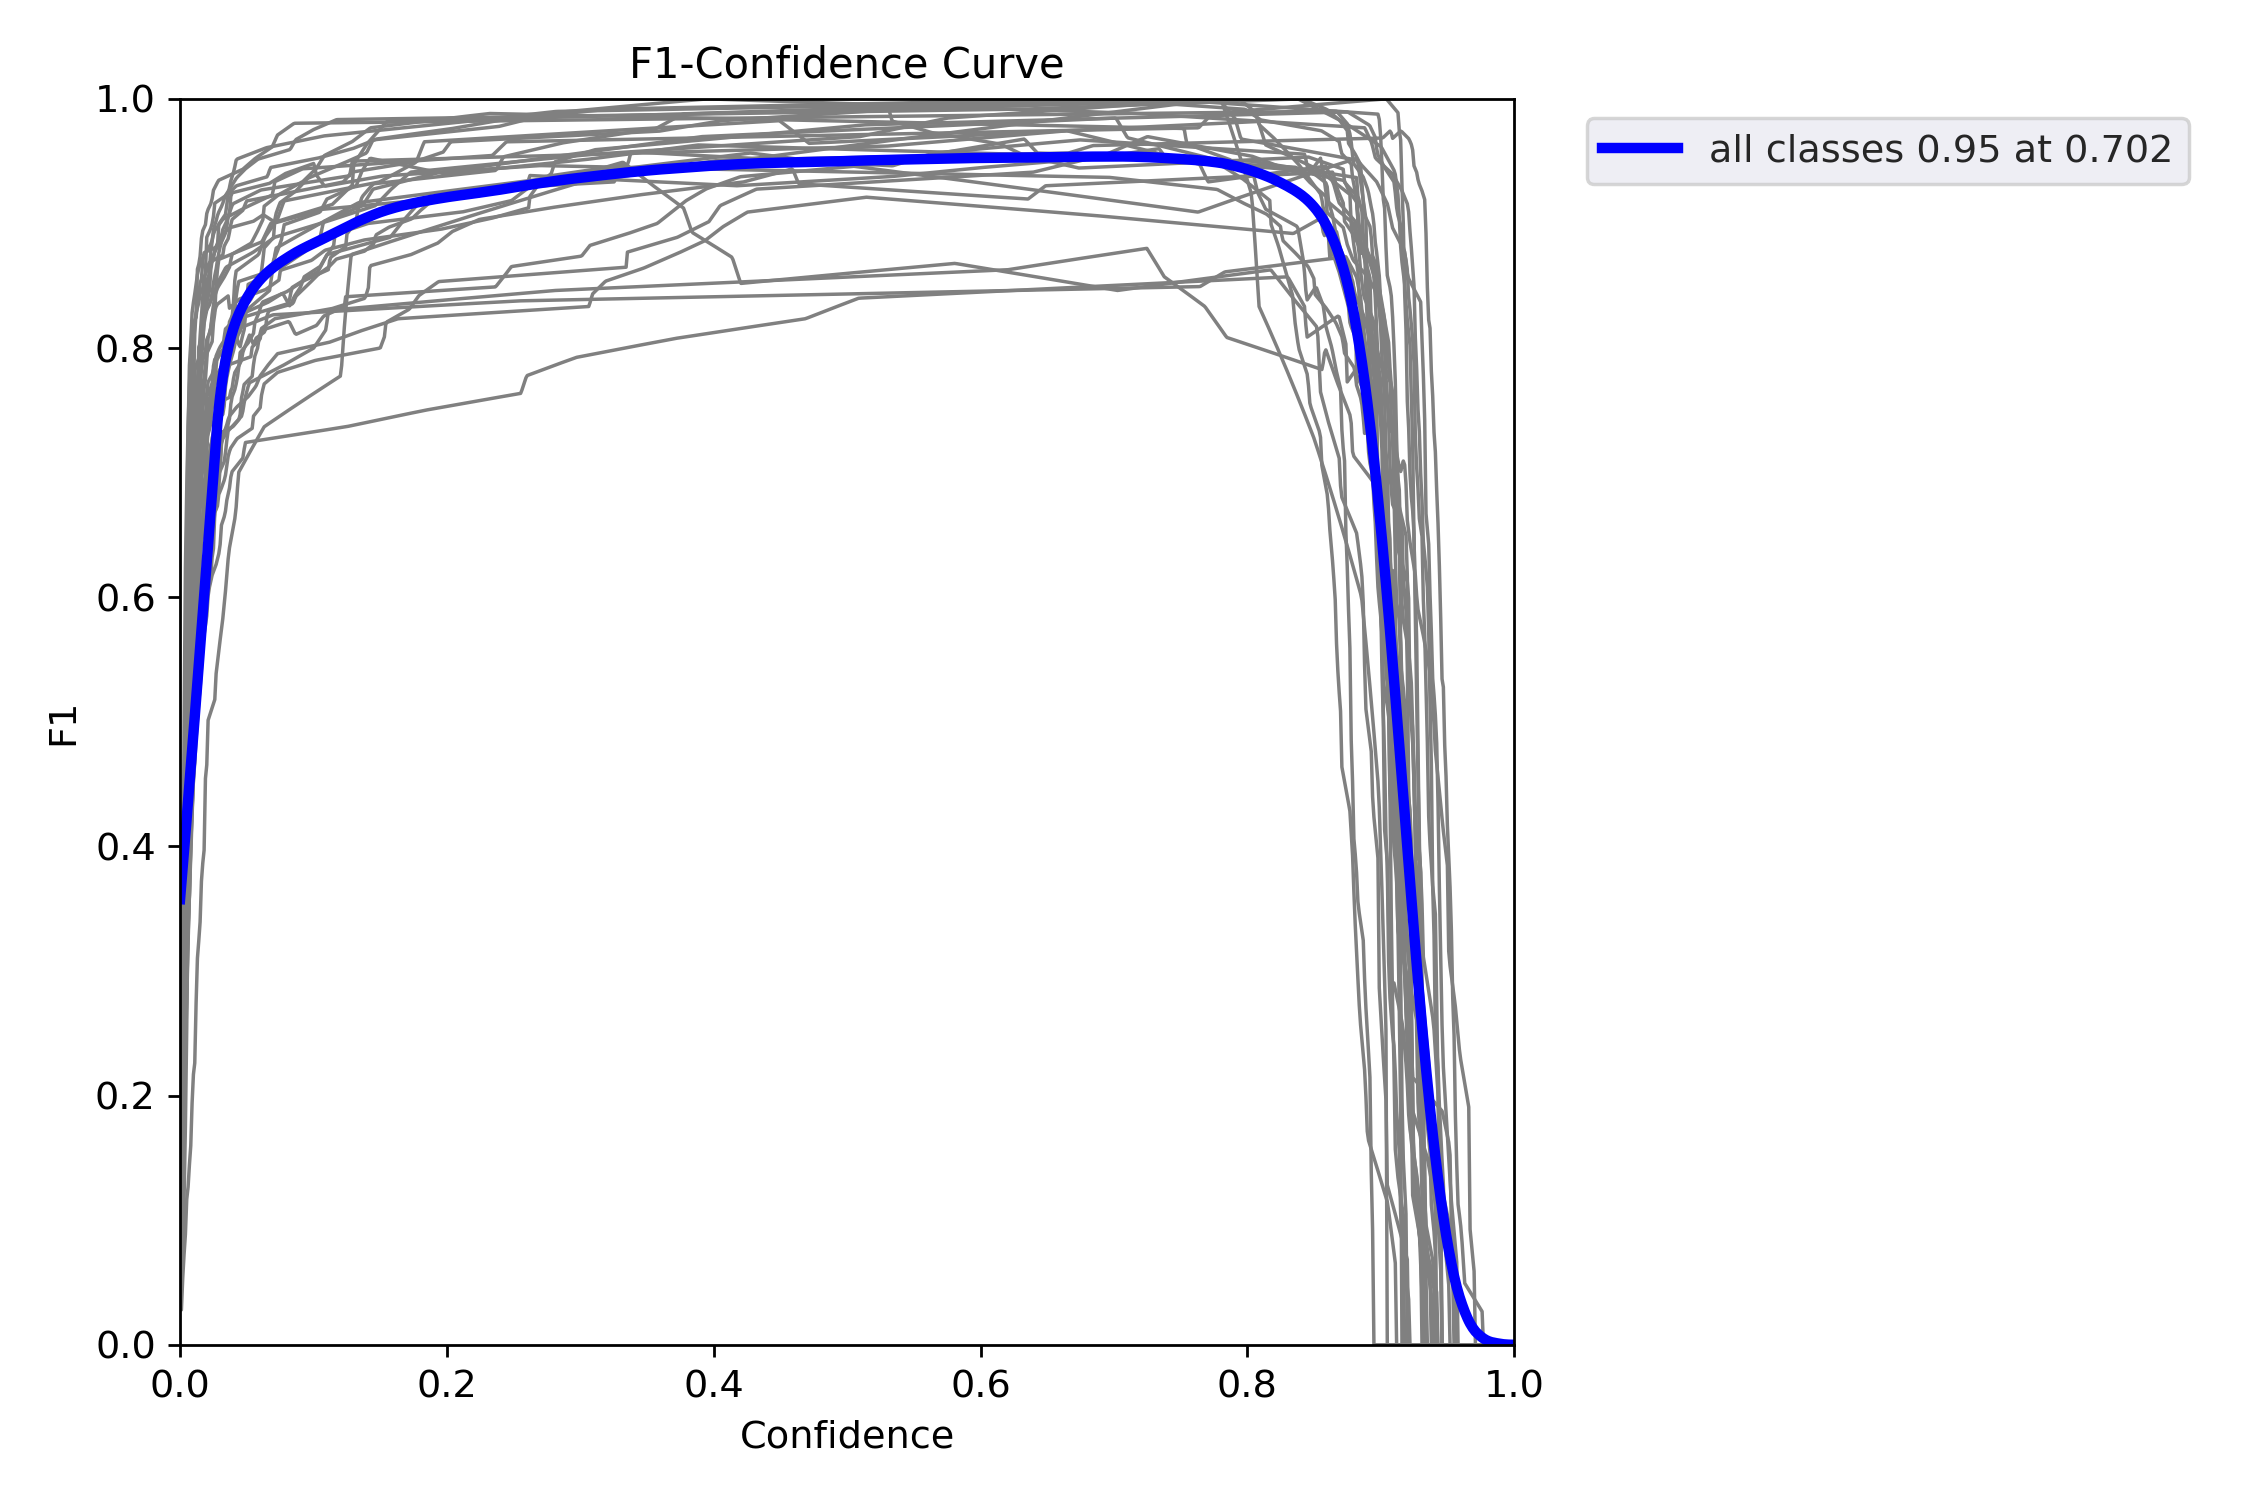
\includegraphics[width=\textwidth]{F1_curve_v5s.png}
        \caption{F1 curve V5s}
        \label{fig:image1}
    \end{subfigure}
    \hfill
    \begin{subfigure}[t]{0.4\textwidth}
        \centering
        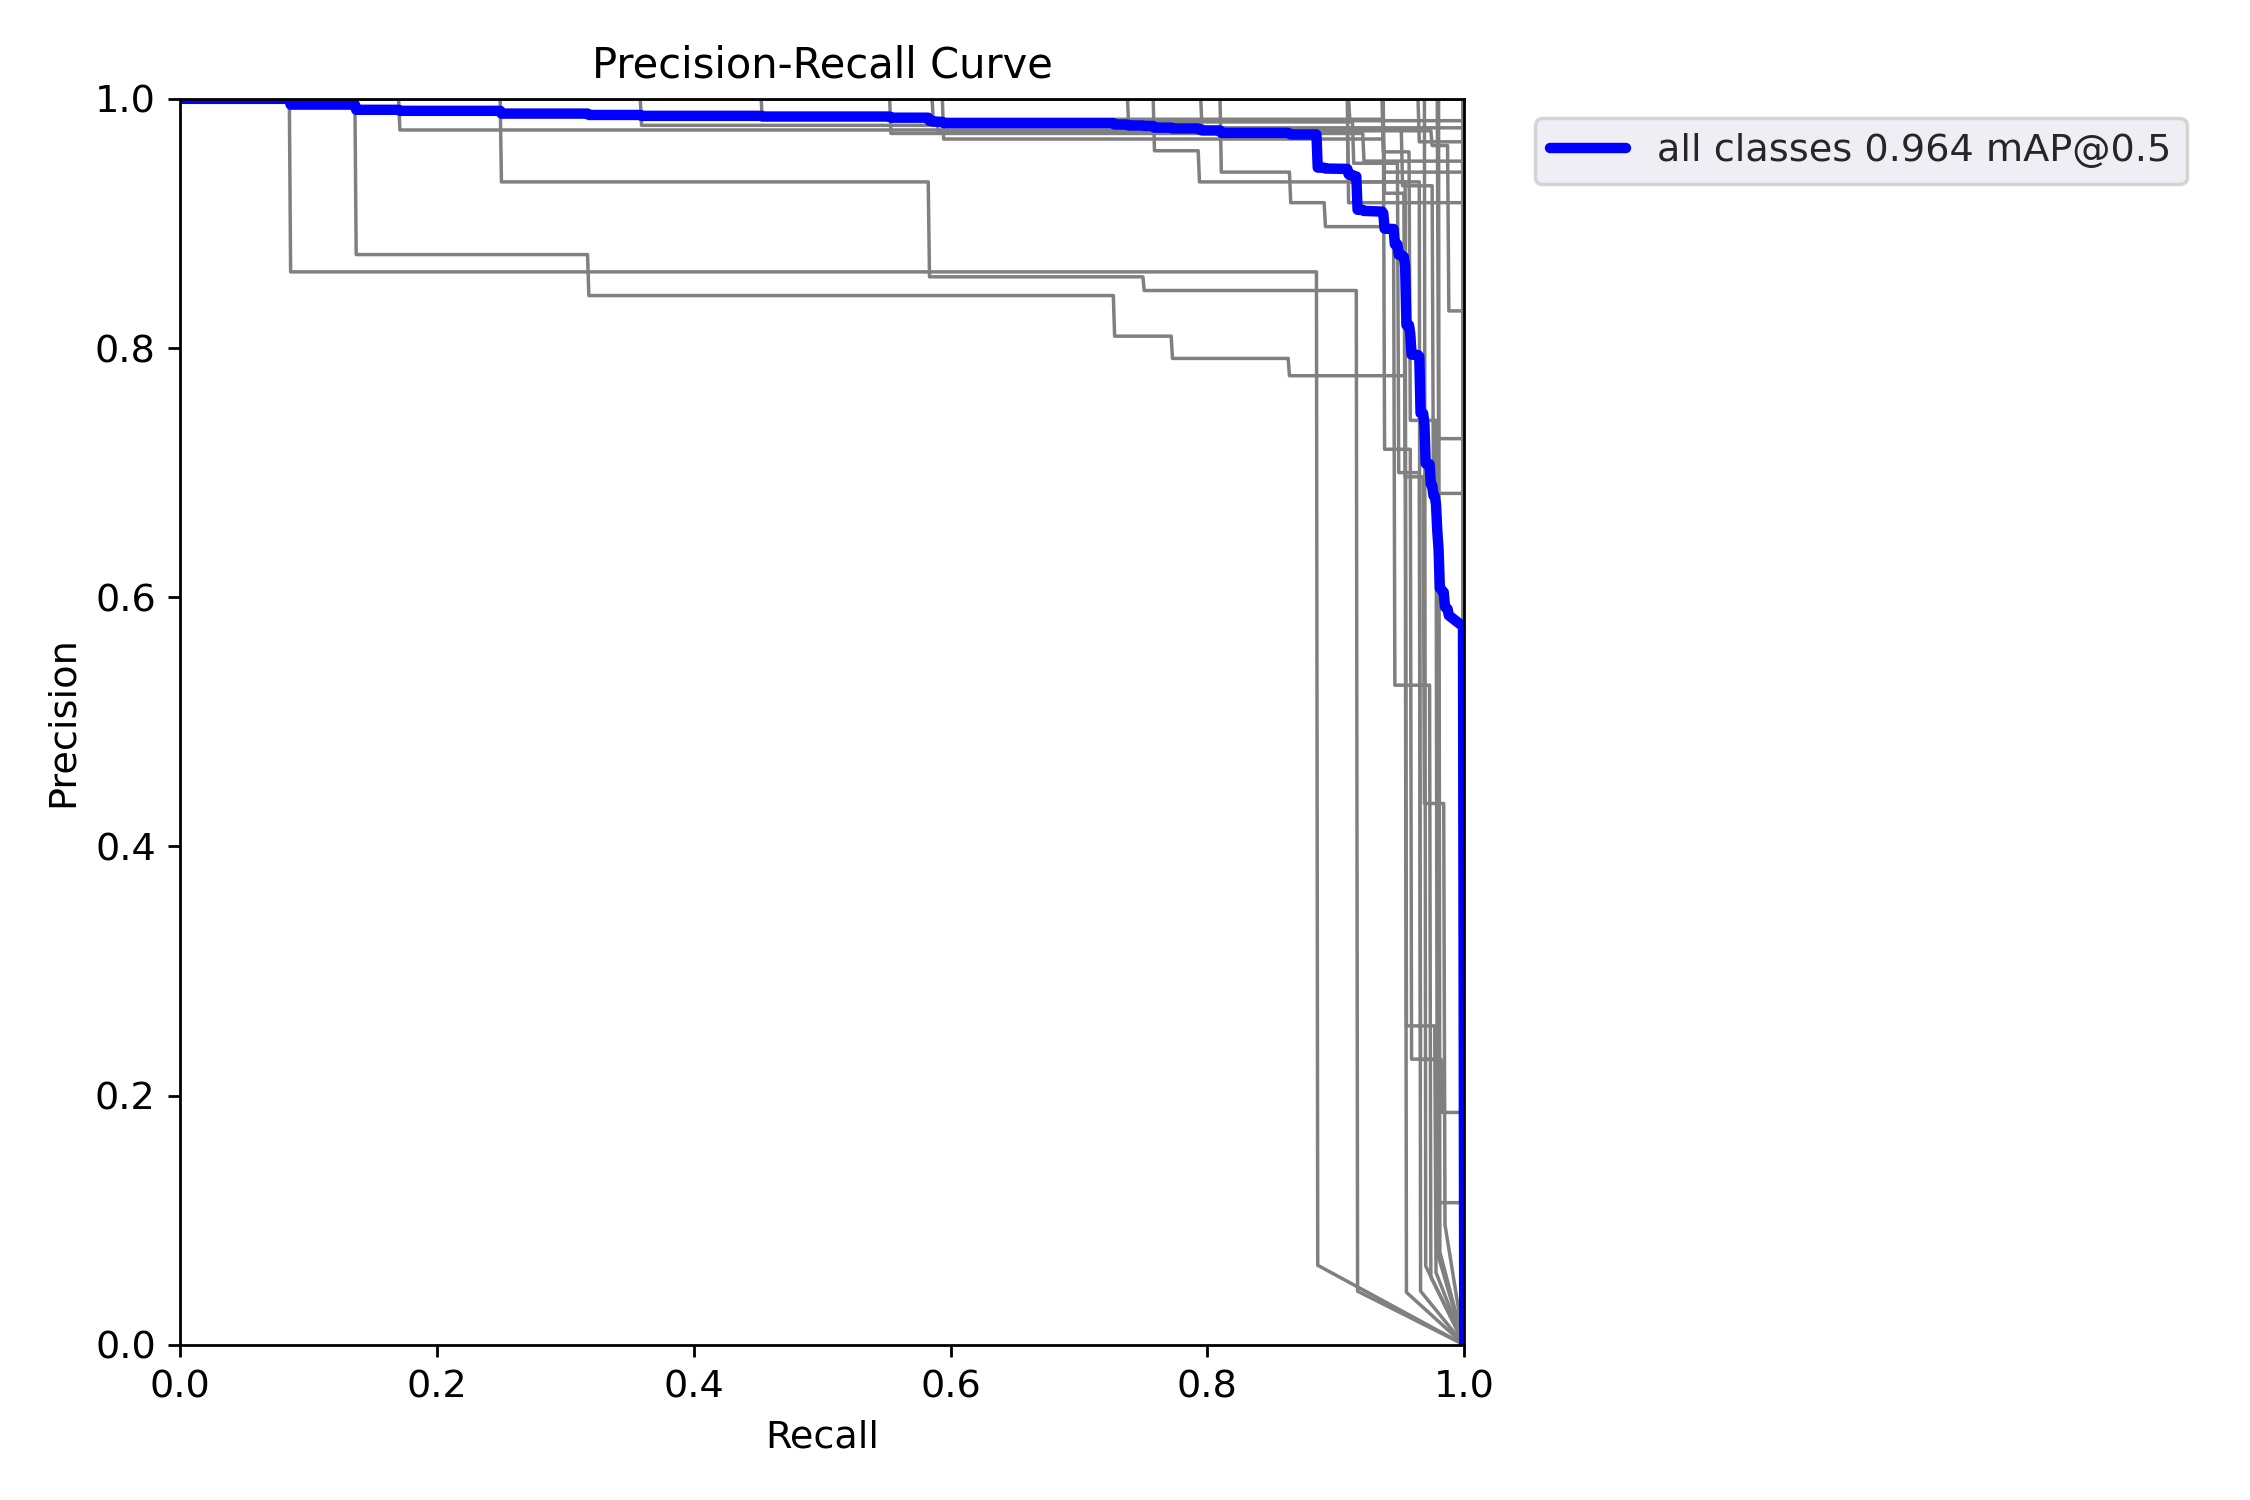
\includegraphics[width=\textwidth]{PR_curve_v5s.png}
        \caption{PR curve V5s}
        \label{fig:image2}
    \end{subfigure}
    \hfill
    \begin{subfigure}[t]{0.4\textwidth}
        \centering
        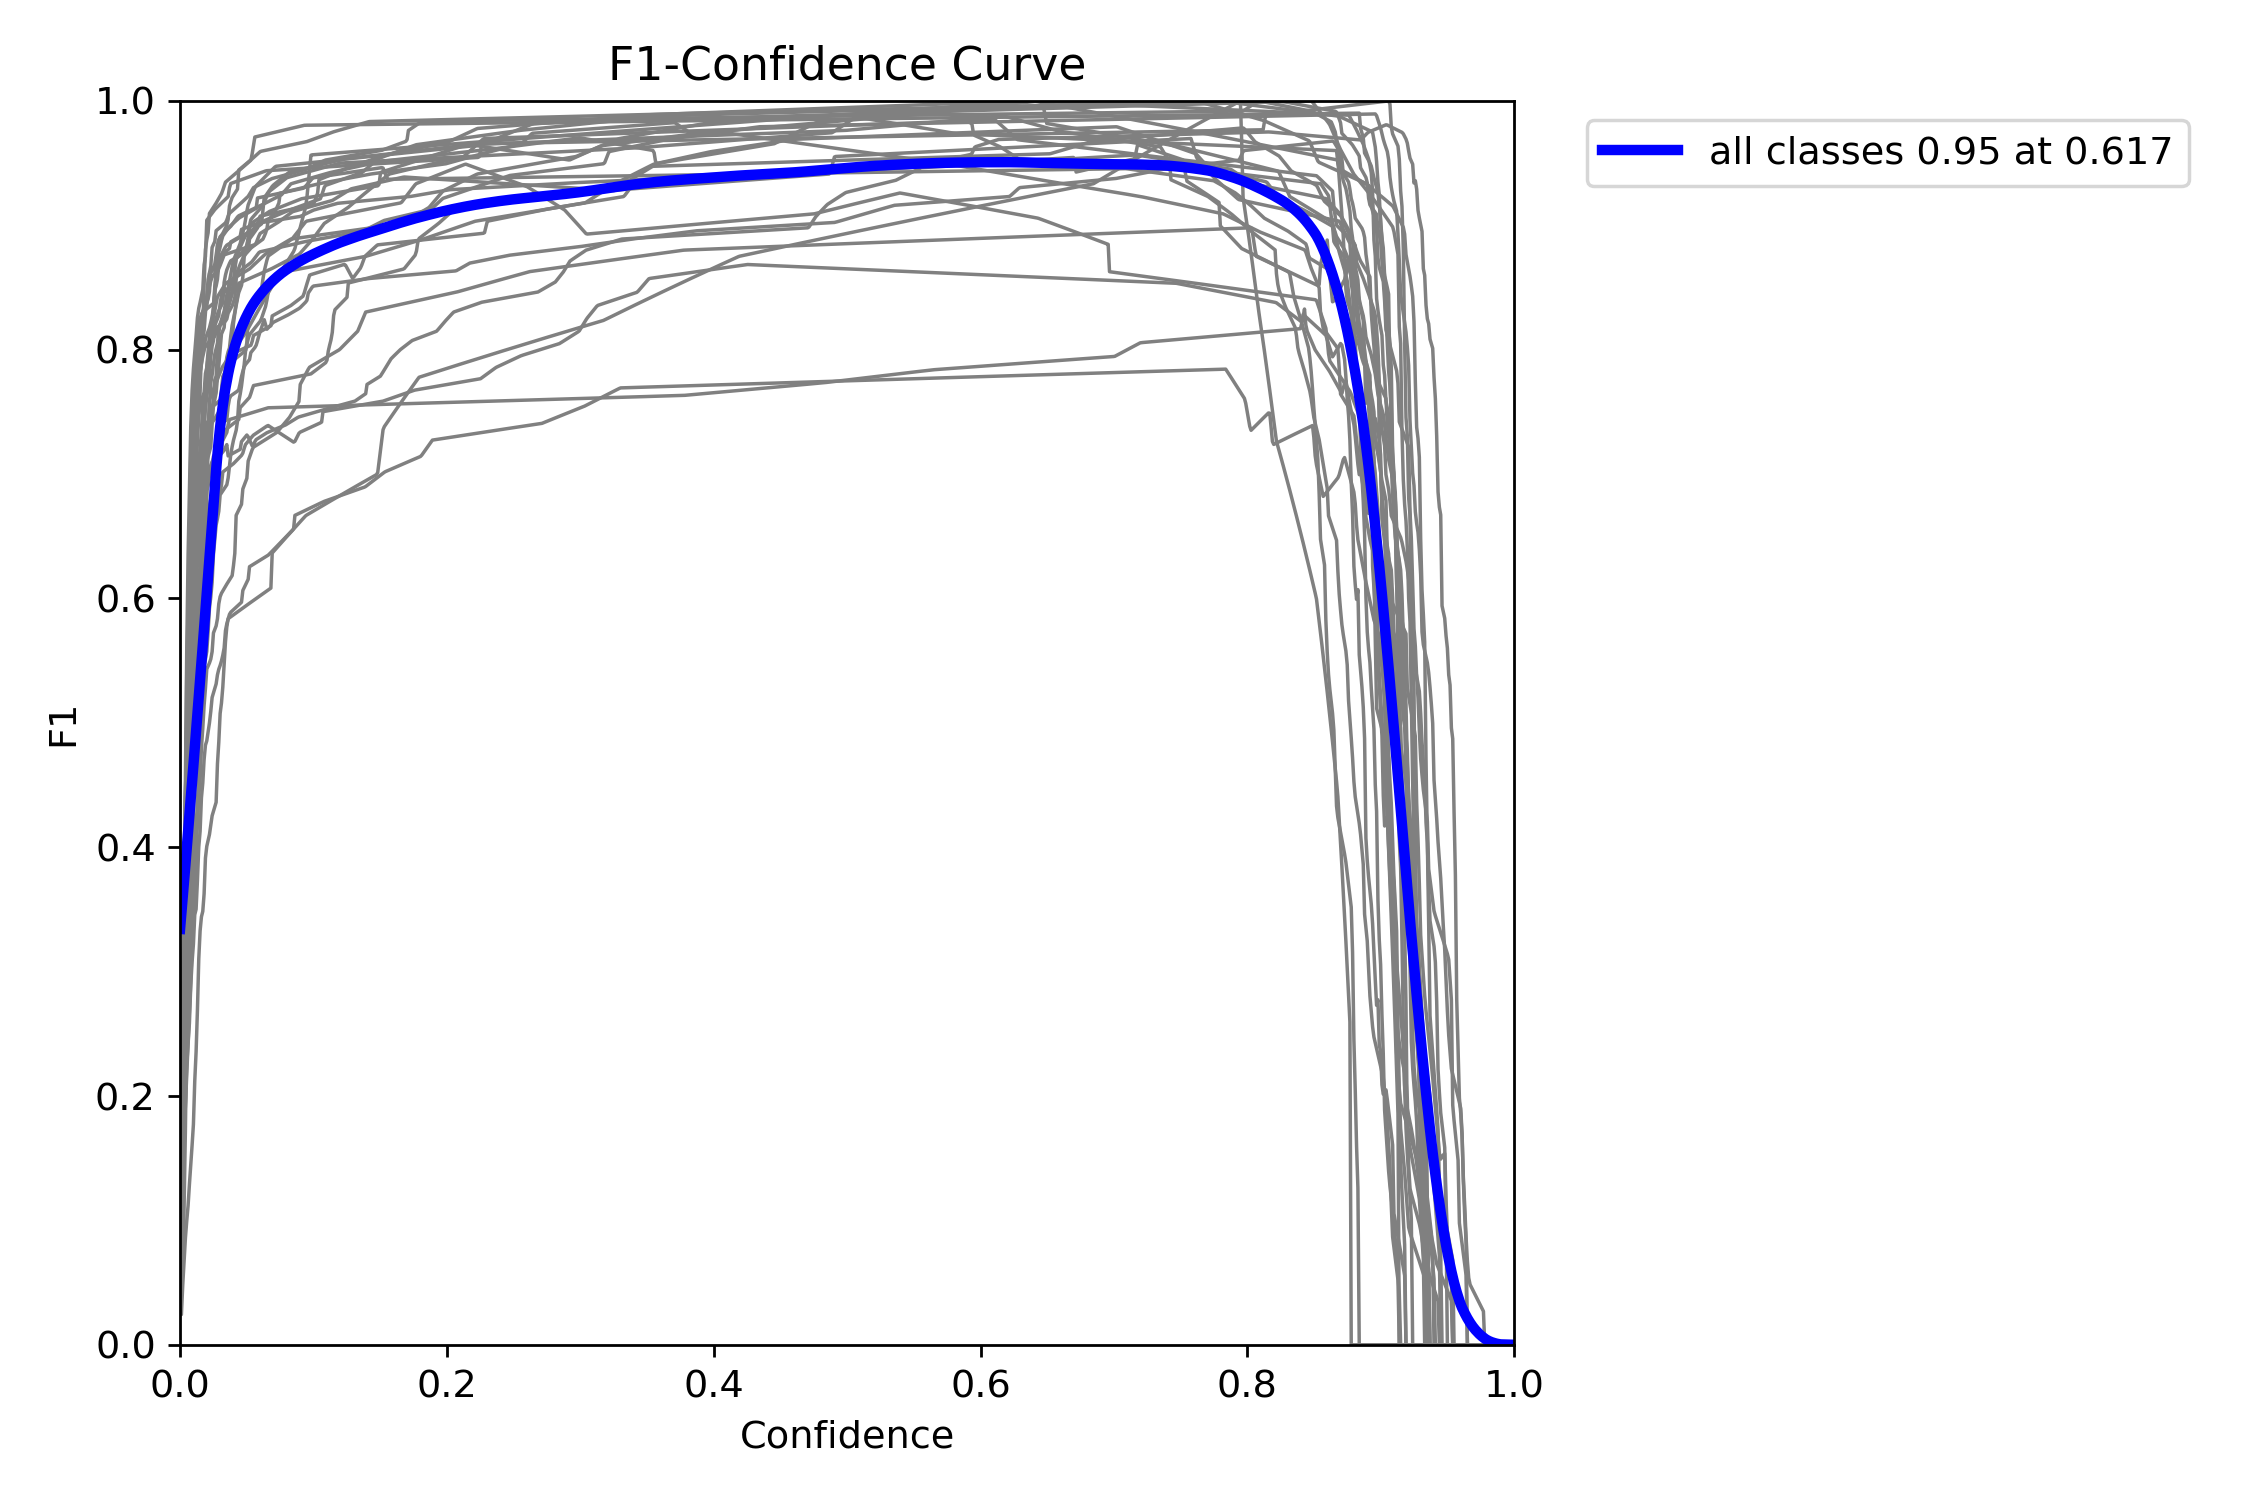
\includegraphics[width=\textwidth]{F1_curve_v5x.png}
        \caption{F1 curve V5x}
        \label{fig:image3}
    \end{subfigure}
    \hfill
    \begin{subfigure}[t]{0.4\textwidth}
        \centering
        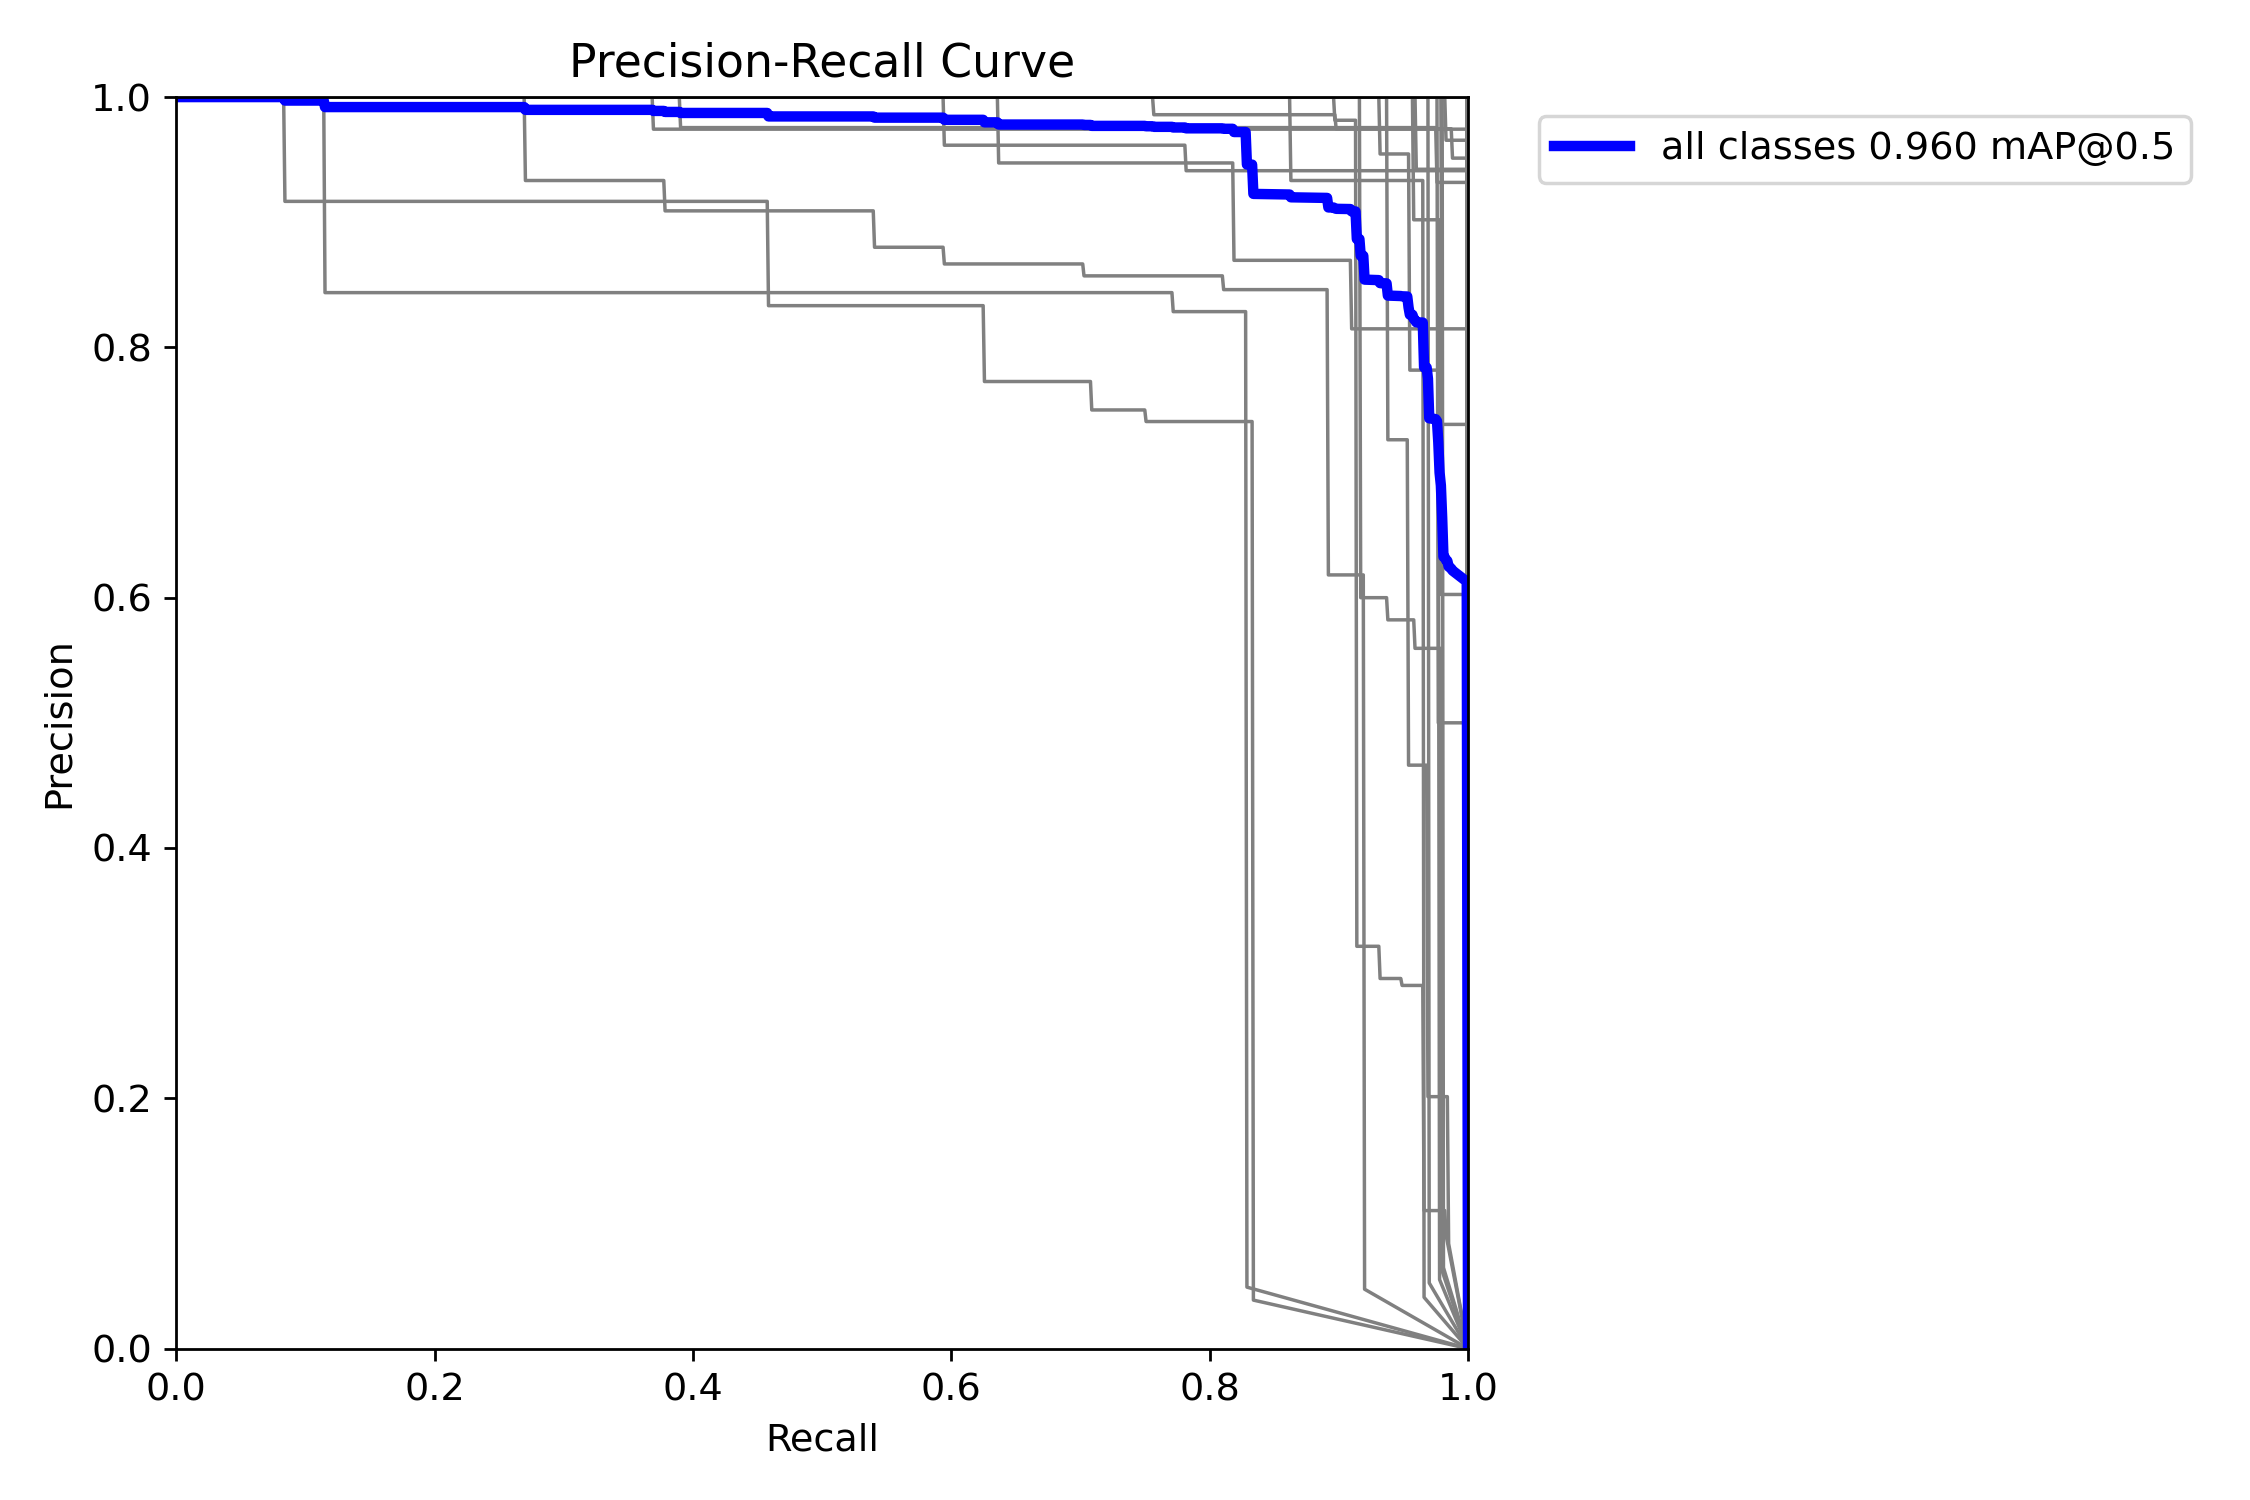
\includegraphics[width=\textwidth]{PR_curve-v5x.png}
        \caption{PR curve V5x}
        \label{fig:image4}
    \end{subfigure}
    
    % Add vertical spacing between rows
    \vspace{0.5cm}
    
    % Second row of images
    \begin{subfigure}[t]{0.4\textwidth}
        \centering
        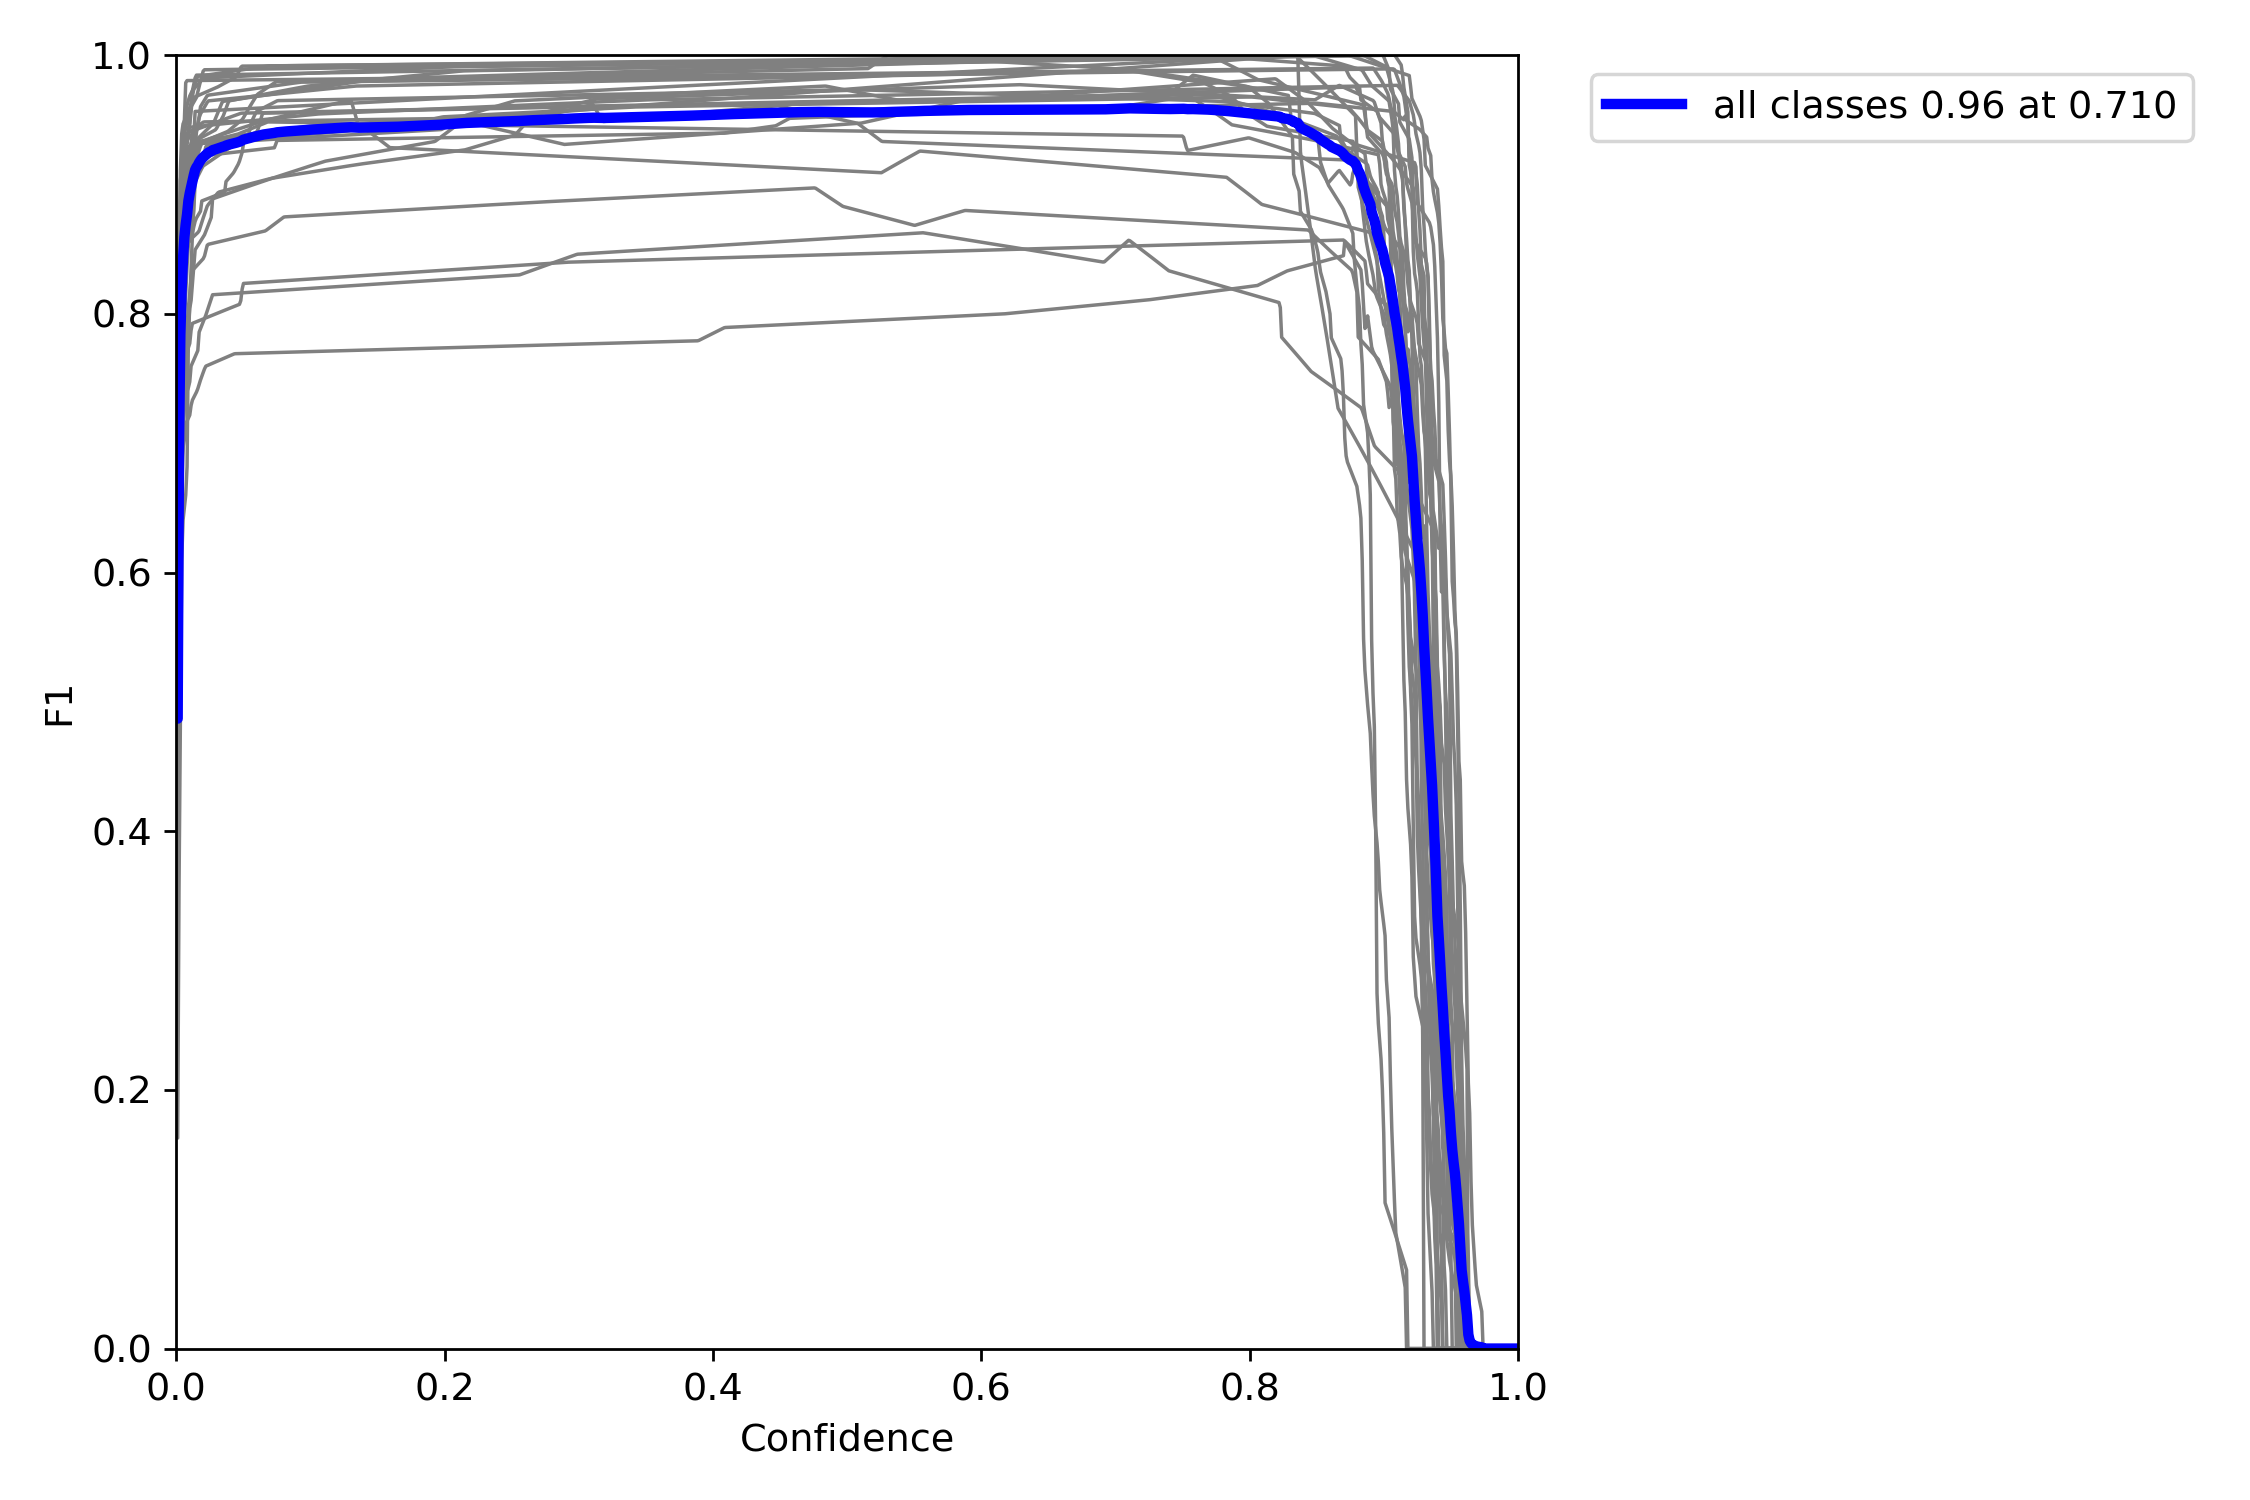
\includegraphics[width=\textwidth]{F1_curve_v7.png}
        \caption{F1 curve V7}
        \label{fig:image5}
    \end{subfigure}
    \hfill
    \begin{subfigure}[t]{0.4\textwidth}
        \centering
        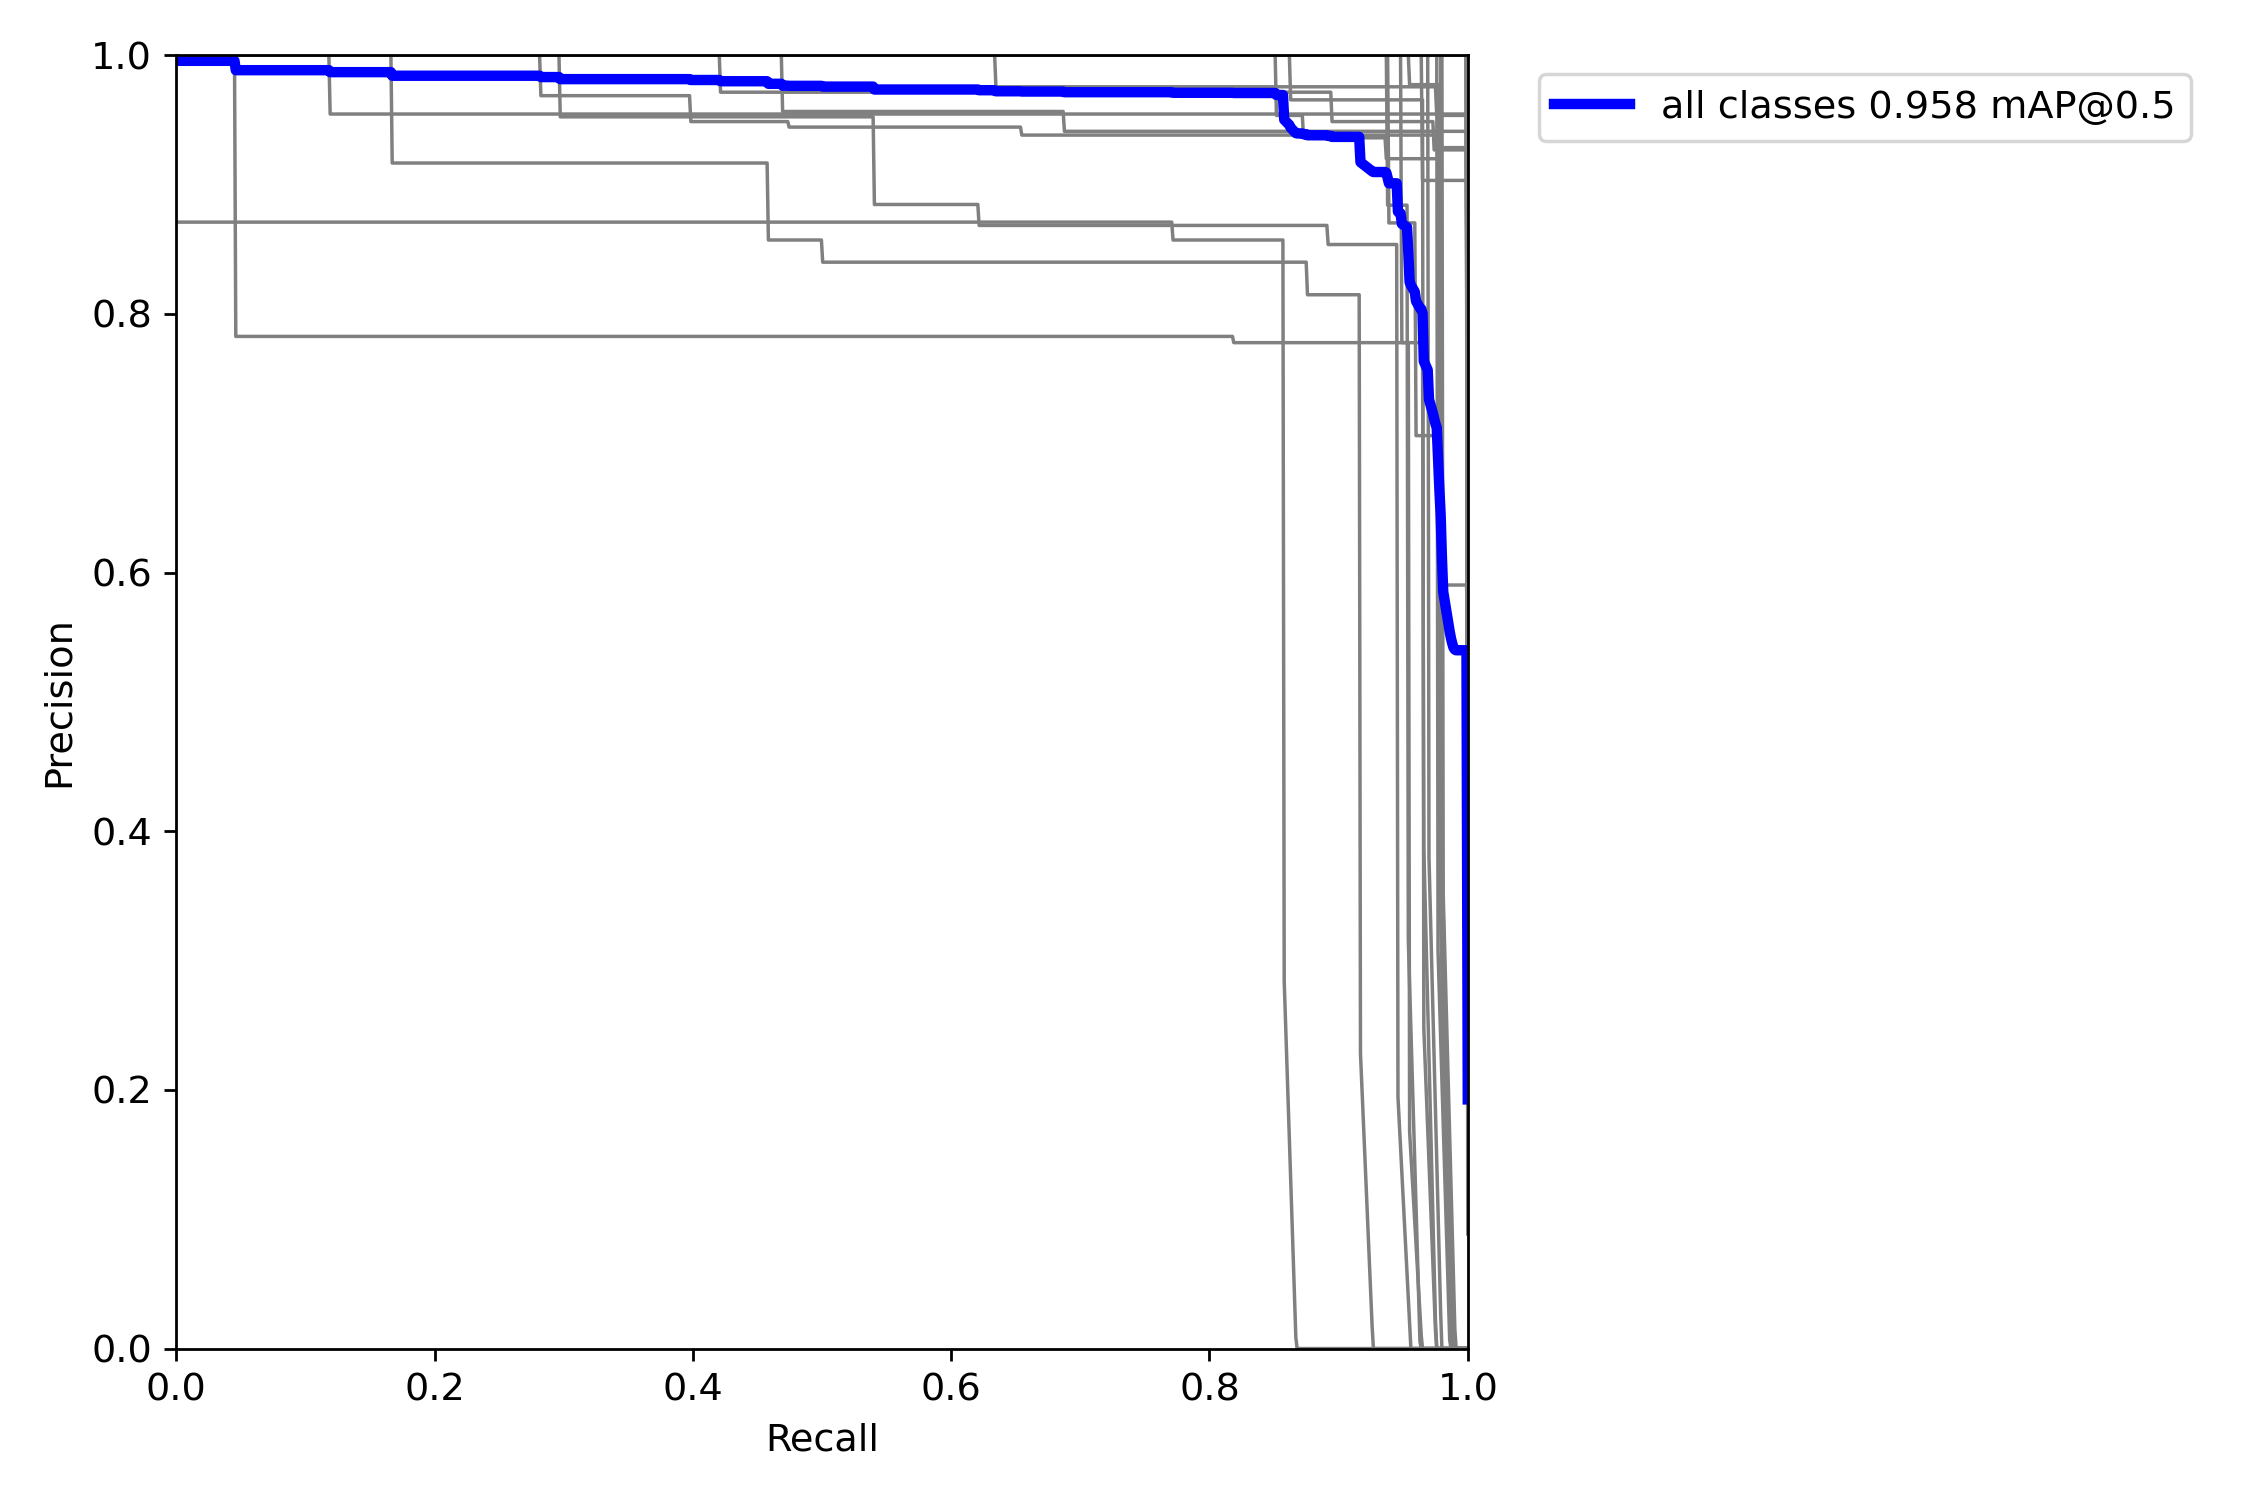
\includegraphics[width=\textwidth]{PR_curve_v7.png}
        \caption{PR curve V7}
        \label{fig:image6}
    \end{subfigure}
    \hfill
    \begin{subfigure}[t]{0.4\textwidth}
        \centering
        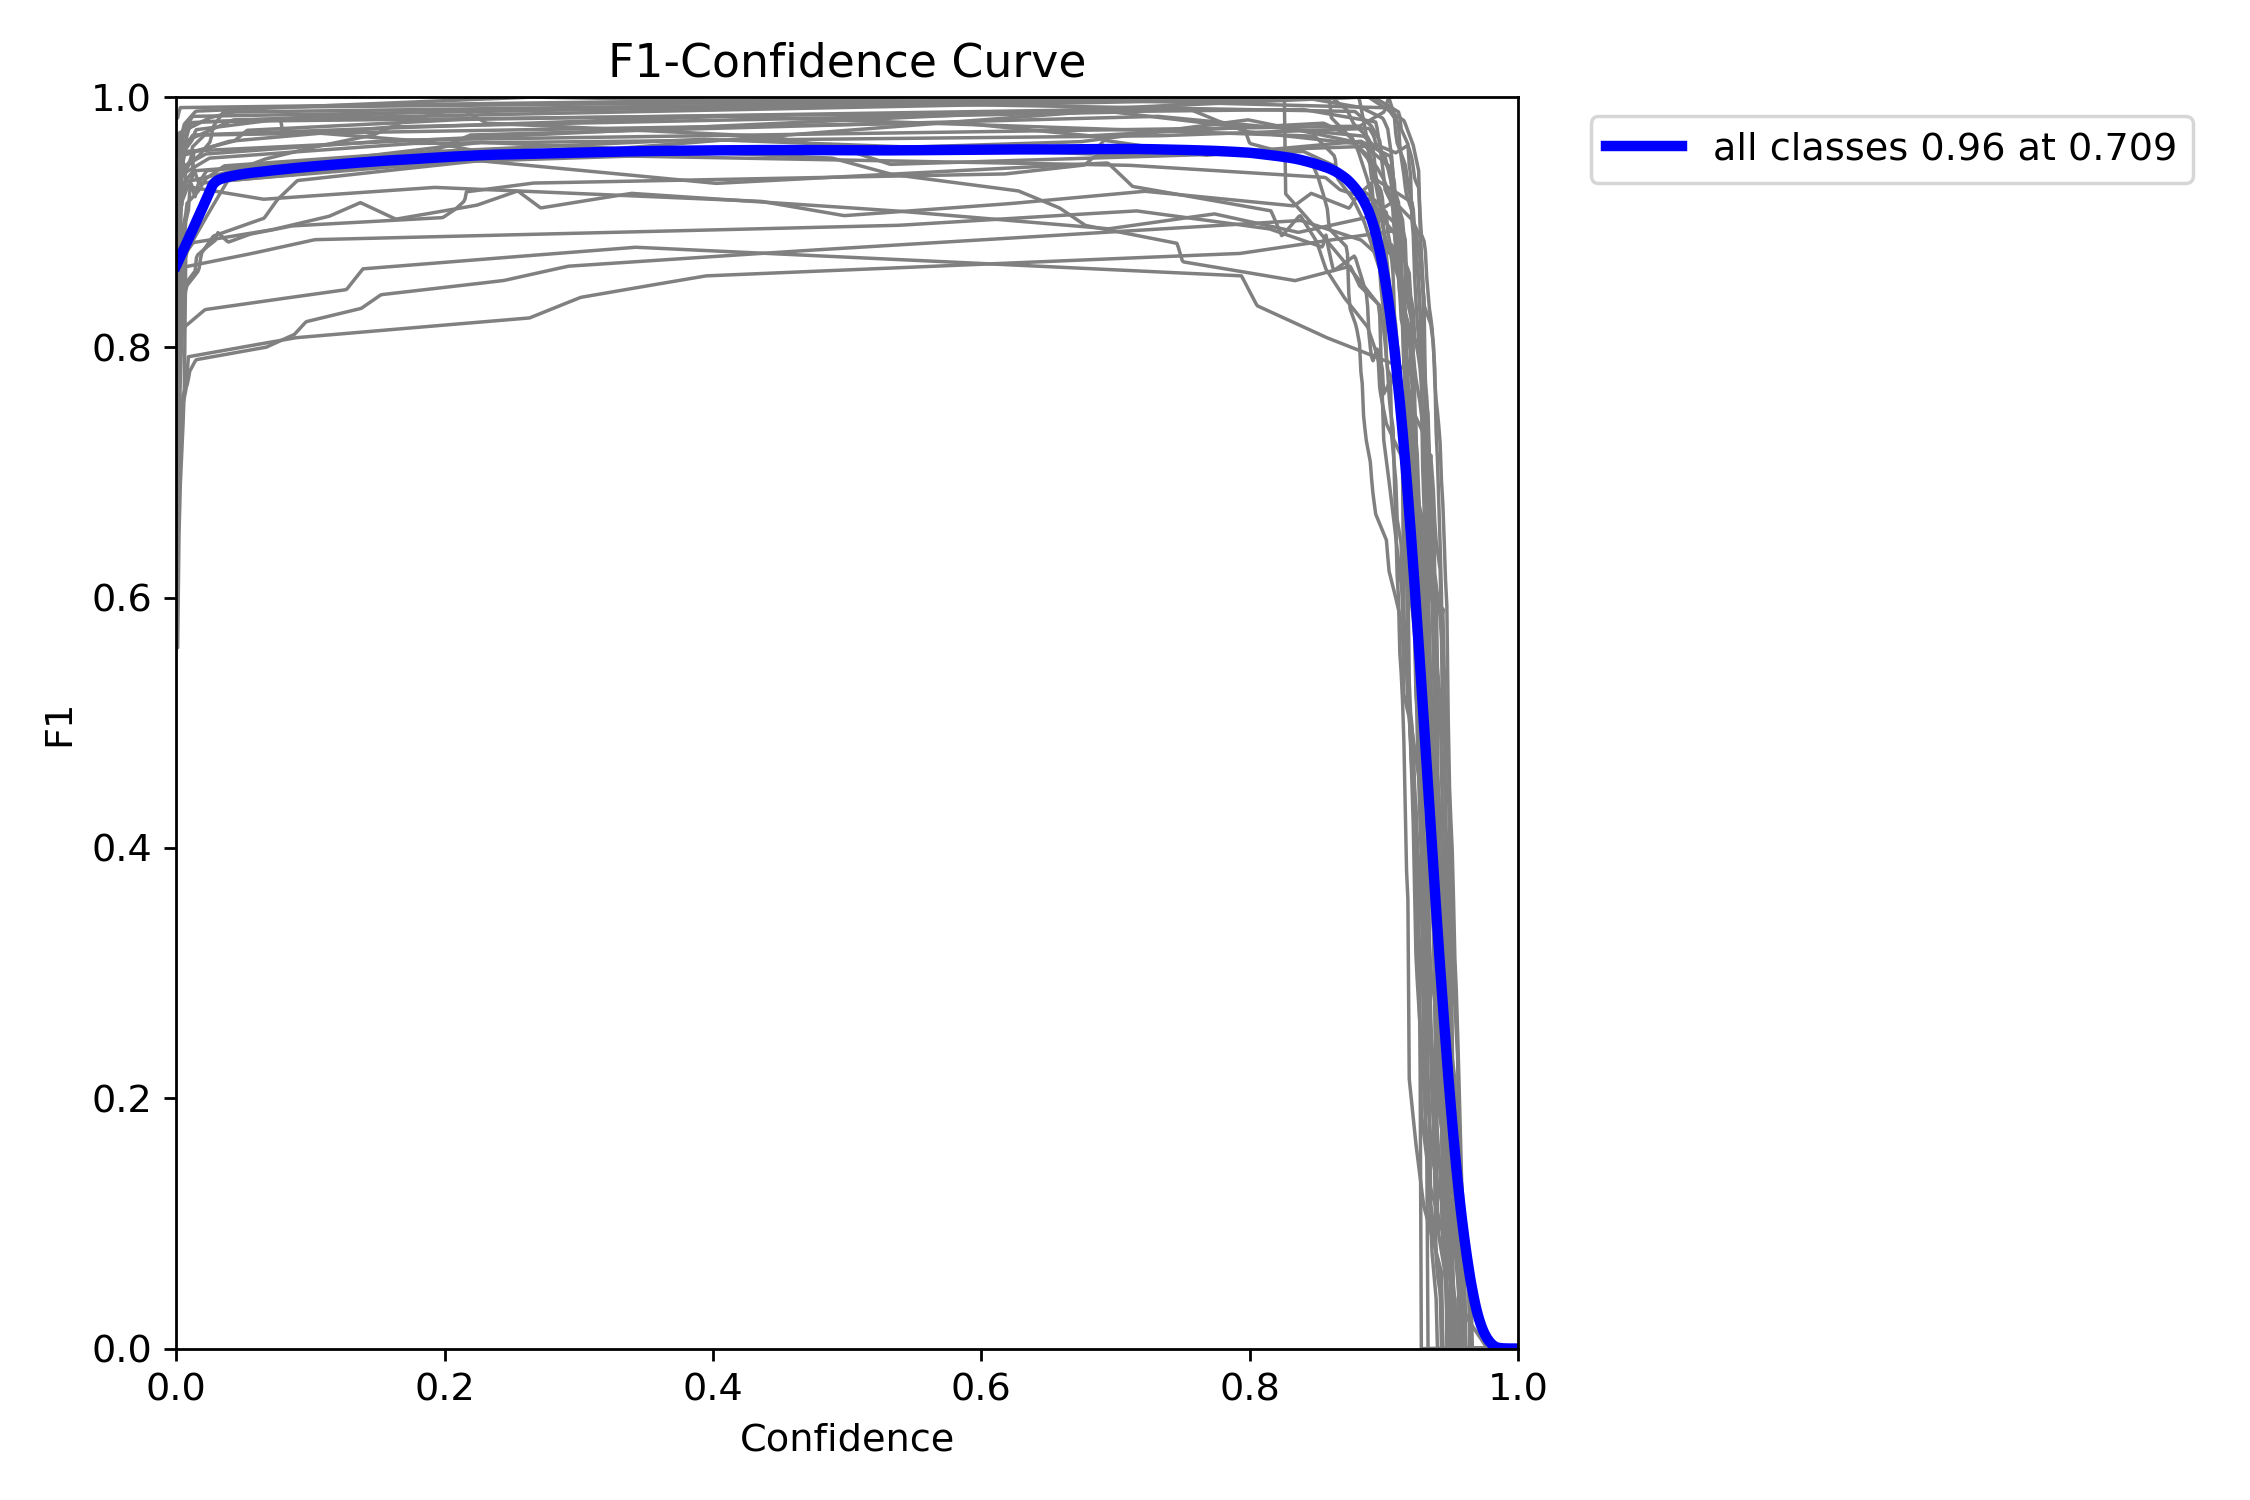
\includegraphics[width=\textwidth]{F1_curve_v8s.png}
        \caption{F1 curve V8s}
        \label{fig:image7}
    \end{subfigure}
    \hfill
    \begin{subfigure}[t]{0.4\textwidth}
        \centering
        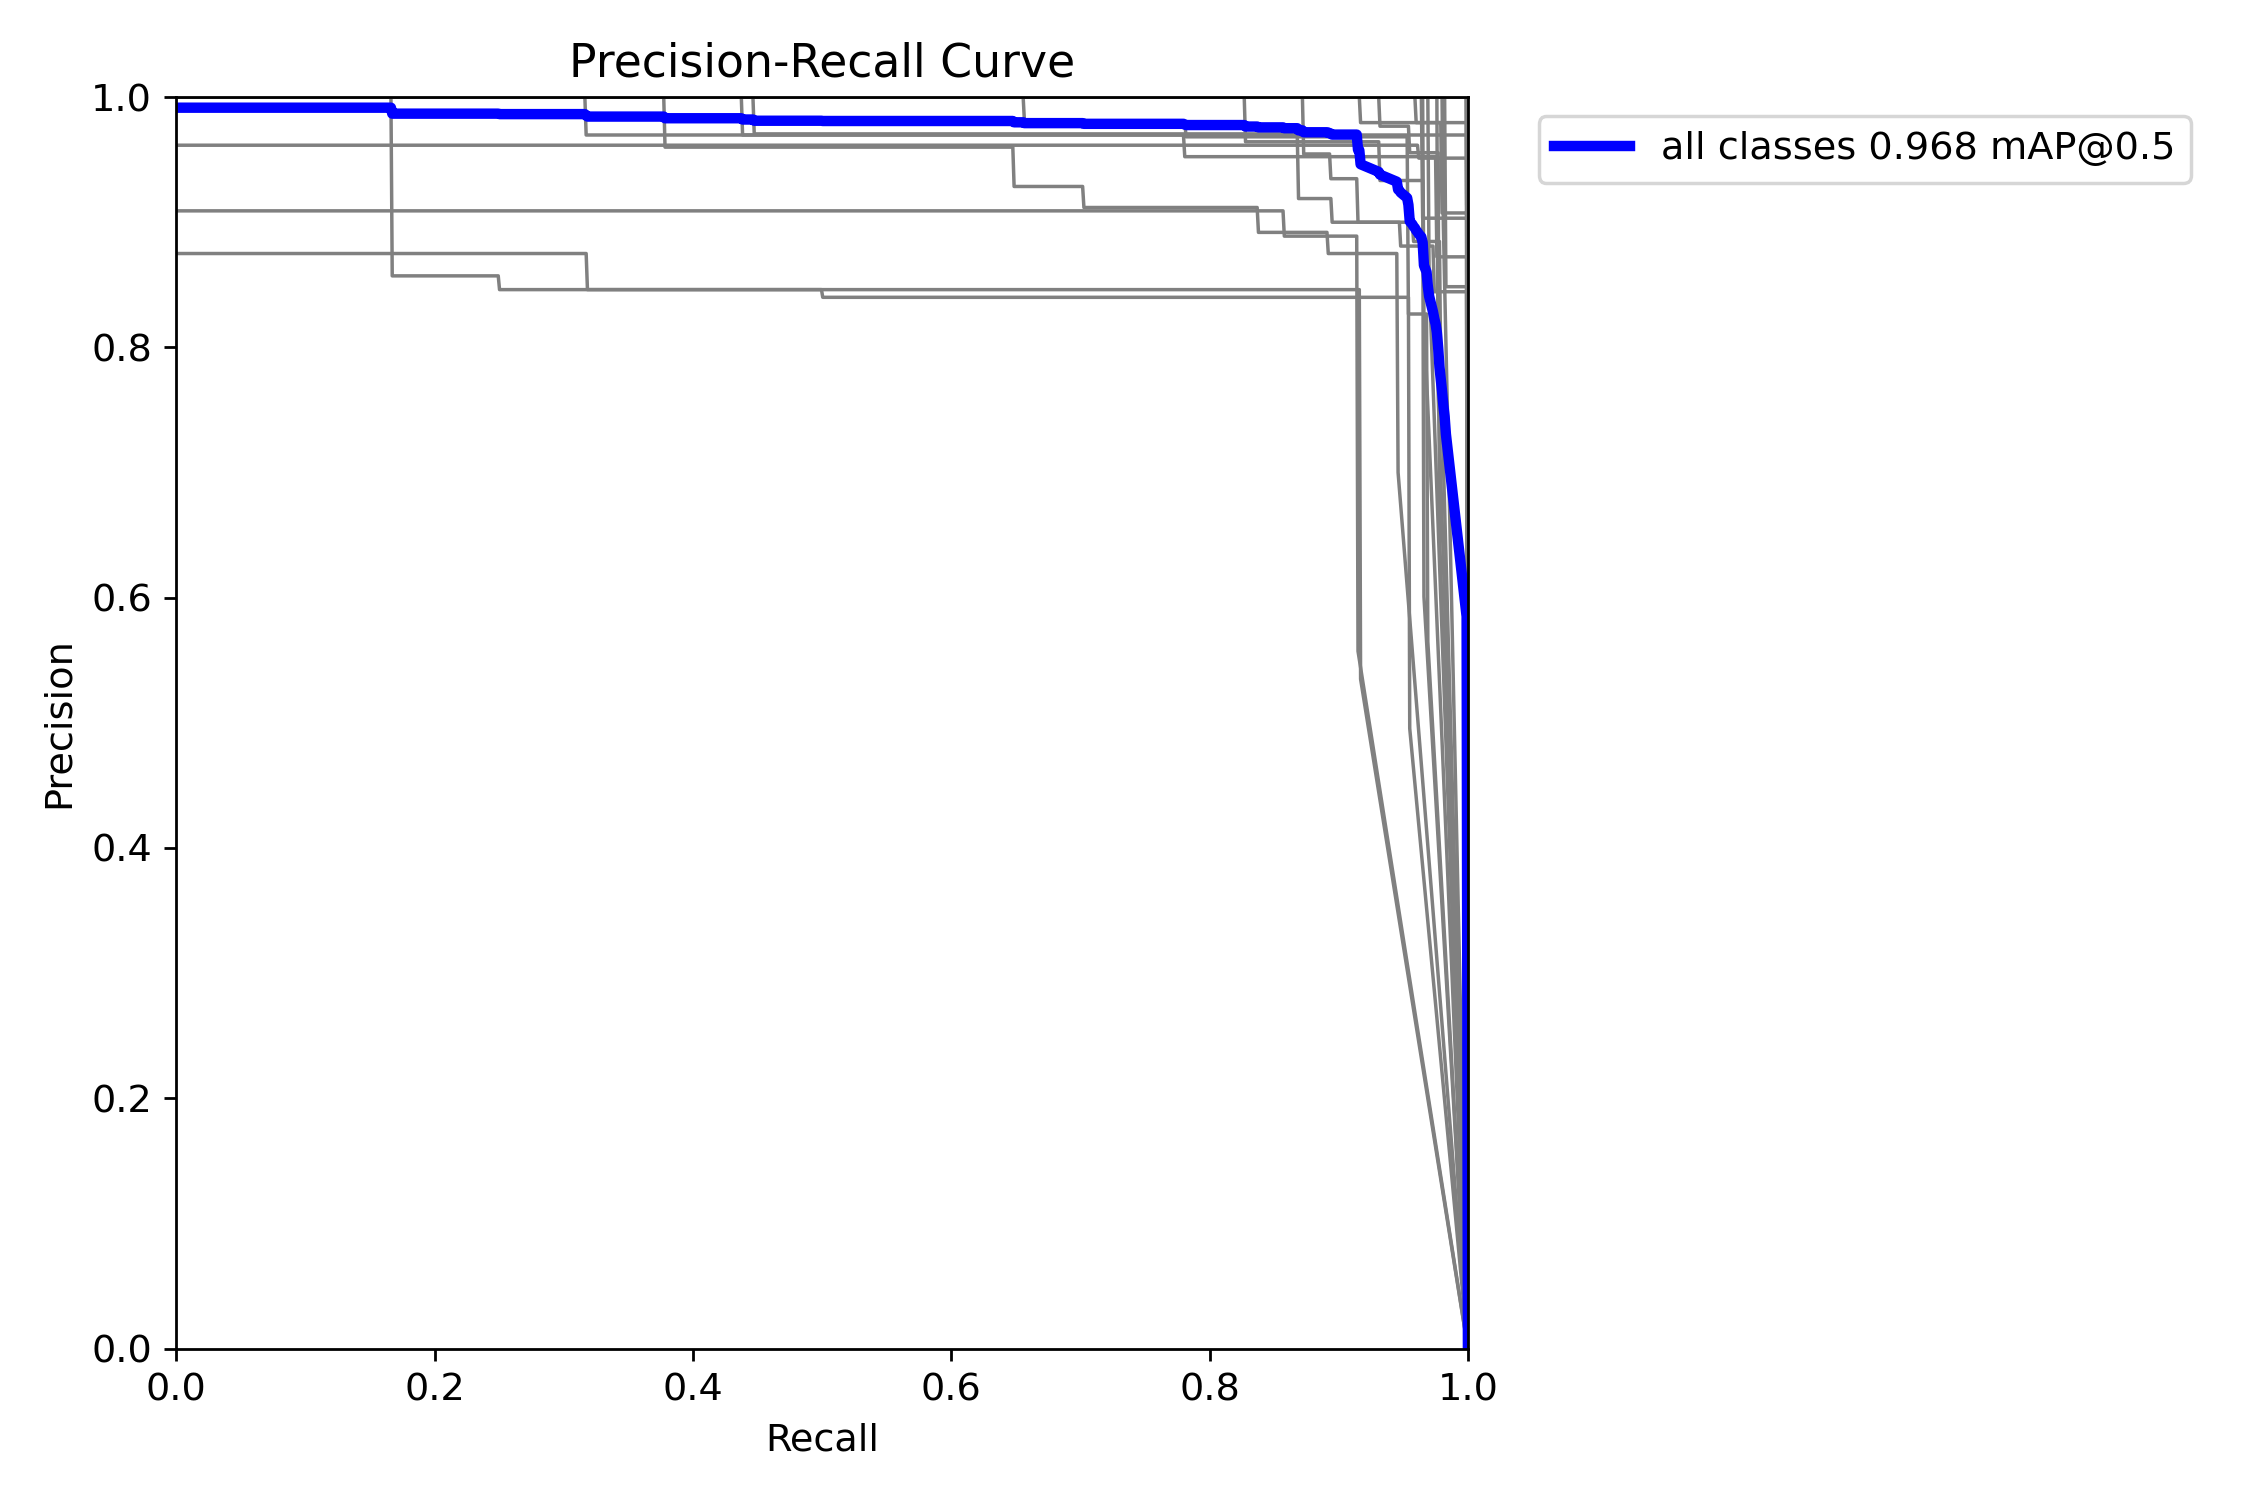
\includegraphics[width=\textwidth]{PR_curve_v8s.png}
        \caption{PR curve V8s}
        \label{fig:image8}
    \end{subfigure}
    
    % Add vertical spacing between rows
    \vspace{0.5cm}
    
    % Third row of images
    \begin{subfigure}[t]{0.4\textwidth}
        \centering
        \includegraphics[width=\textwidth]{F1_curve_v8X.png}
        \caption{F1 curve V8X}
        \label{fig:image9}
    \end{subfigure}
    \hfill
    \begin{subfigure}[t]{0.4\textwidth}
        \centering
        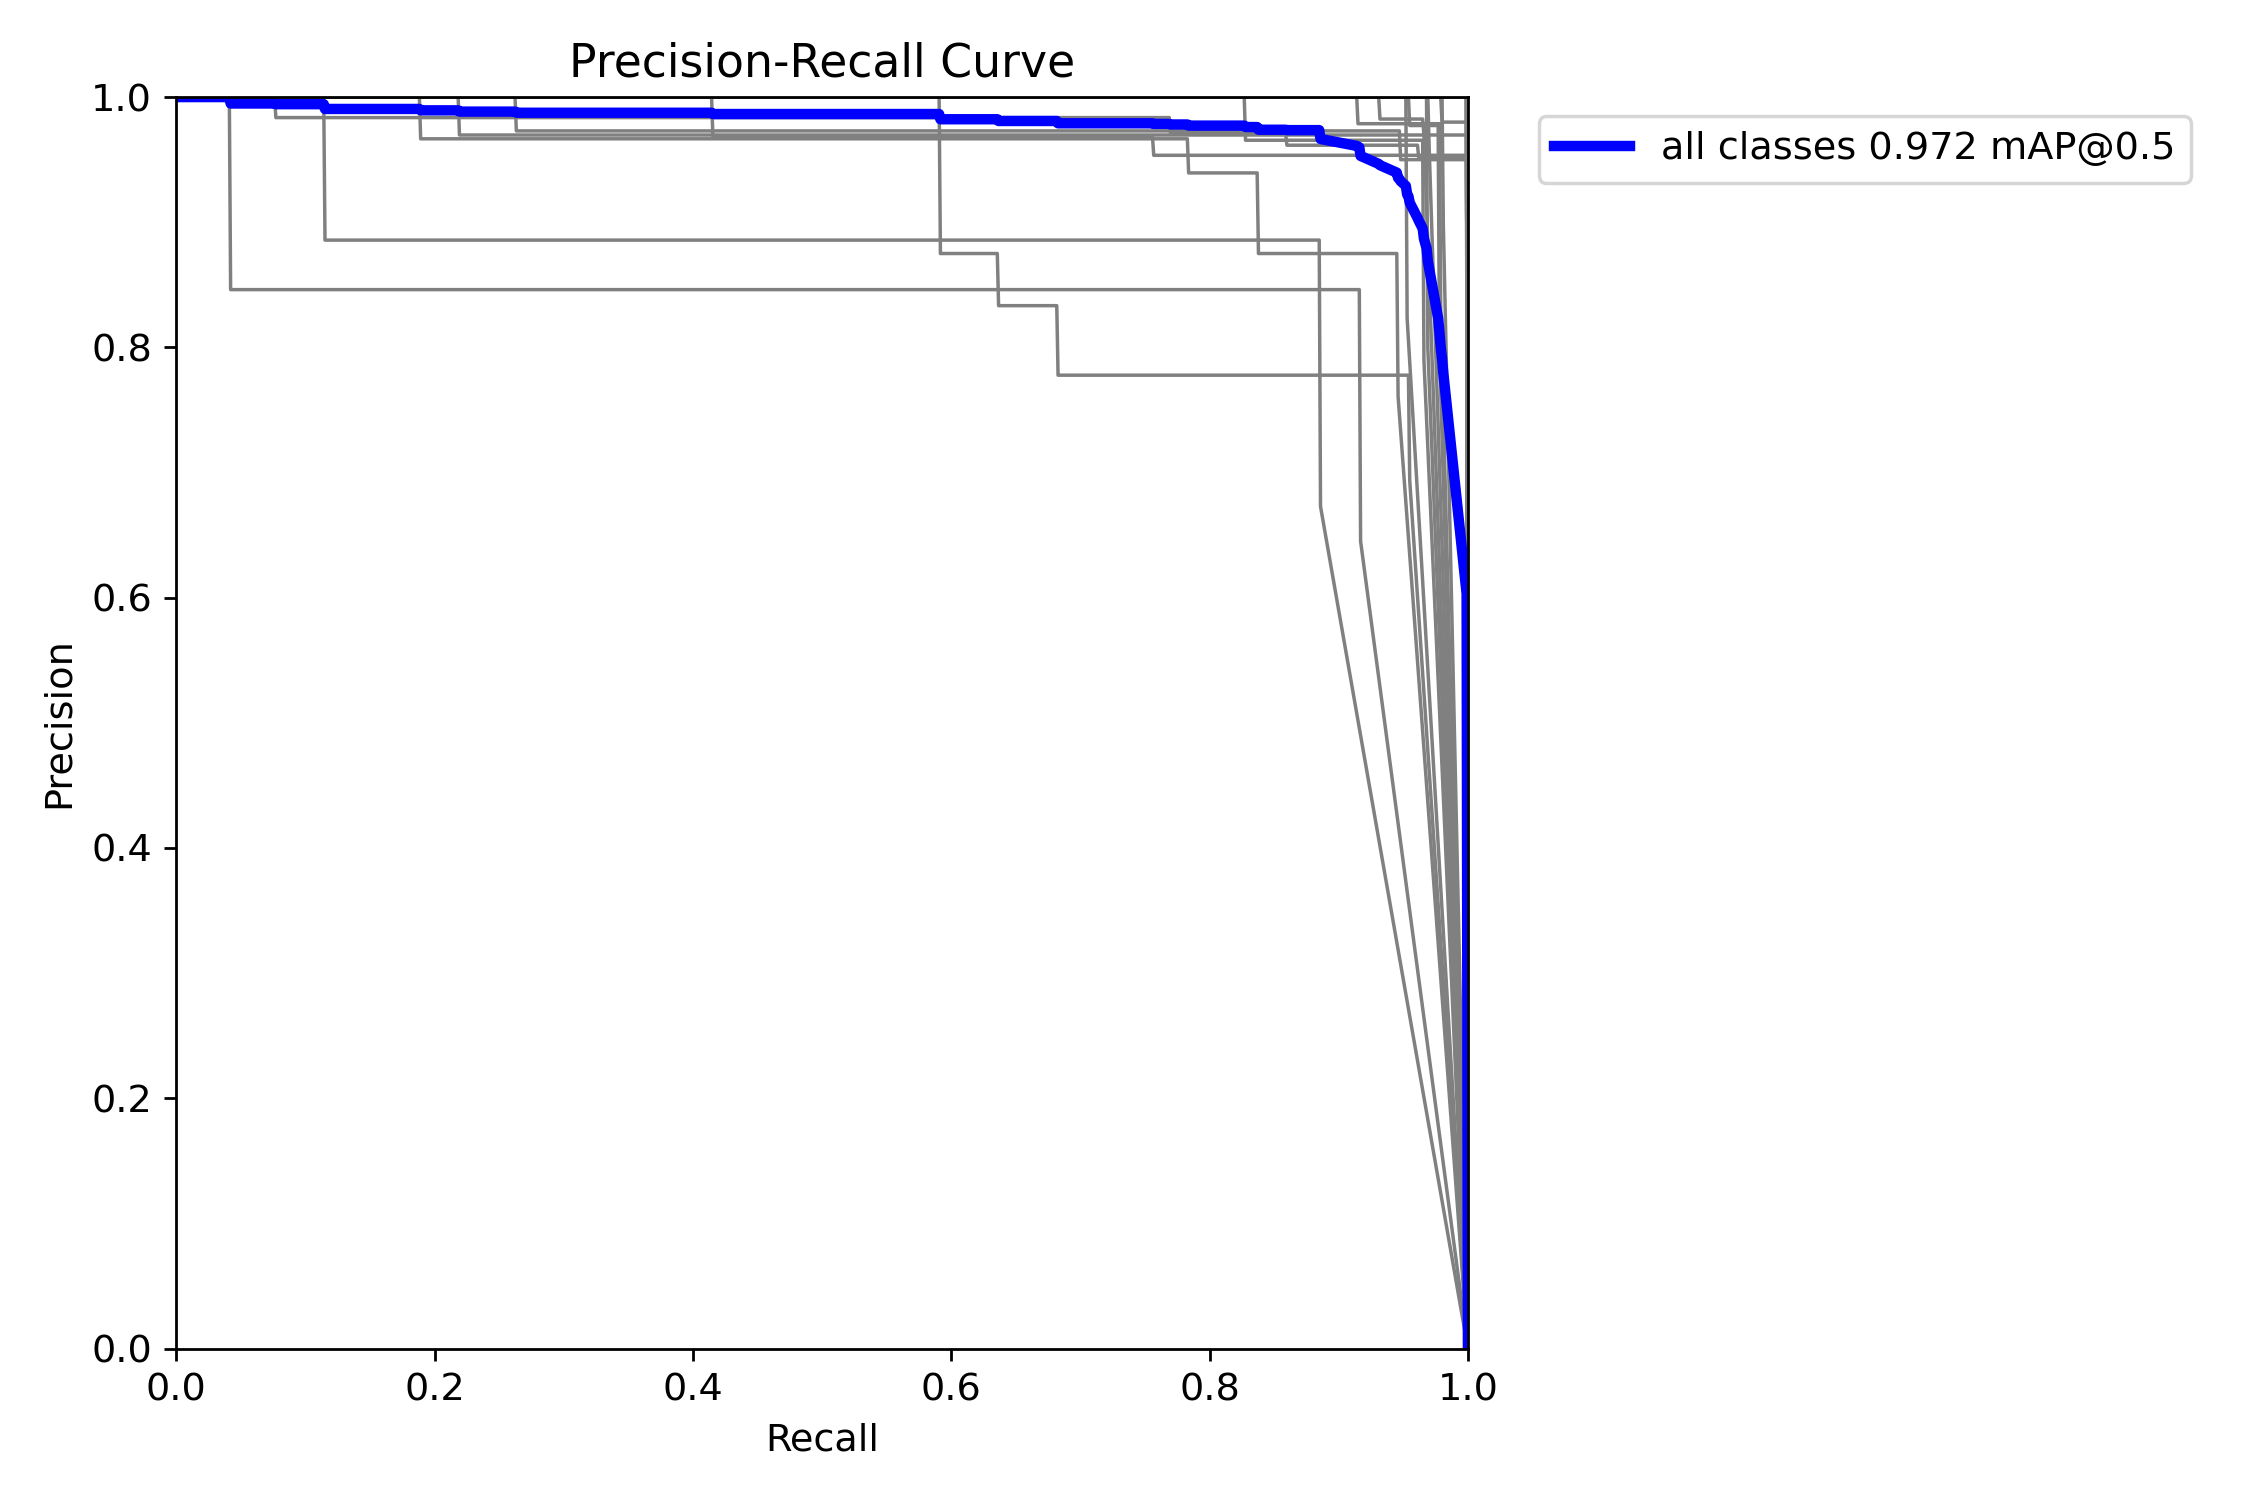
\includegraphics[width=\textwidth]{PR_curve_v8x.png}
        \caption{PR curve V8x}
        \label{fig:image10}
    \end{subfigure}
    
    \caption{F1 CURVE AND PR CURVE OF MODELS}
    \label{fig:result_grid}
\end{figure}



\subsection{Outline of Object Detection Models}
To identify the optimal object detection model for ingredient recognition in refrigerator images, we evaluated five YOLO (You Only Look Once) variants. These models represent incremental improvements in object detection technology and were trained under identical conditions to ensure a fair comparison. 
\subsubsection{Overview of YOLO Variants}
YOLO models are renowned for their efficiency and real-time performance in object detection tasks. Below, we provide detailed insights into the architectures and advancements of the variants evaluated:

\paragraph{1. YOLOv5 (s and x Variants)}
\begin{itemize}
    \item YOLOv5 introduced several architectural improvements over YOLOv4, including:
          \begin{itemize}
              \item Use of the CSPDarknet53 backbone for enhanced feature extraction.
              \item Mosaic data augmentation to improve model generalization.
              \item An improved anchor-based detection mechanism for precise bounding box localization.
          \end{itemize}
    \item The \texttt{s} (small) variant is designed for computational efficiency, using fewer parameters, making it suitable for edge devices.
    \item The \texttt{x} (extra-large) variant increases the number of layers and parameters, prioritizing accuracy over speed.
    \item Both variants demonstrated reliable performance but struggled to match the accuracy of more recent models like YOLOv8.
\end{itemize}

\paragraph{2. YOLOv7}
\begin{itemize}
    \item YOLOv7 builds upon YOLOv4 and introduces Extended Efficient Layer Aggregation Networks (E-ELAN), which:
          \begin{itemize}
              \item Enhance the learning capacity of the model without significantly increasing computational overhead.
              \item Allow better utilization of feature maps for complex object detection tasks.
          \end{itemize}
    \item This version achieves a superior balance between inference speed and detection accuracy compared to YOLOv5.
    \item YOLOv7 performs exceptionally well in scenarios requiring high precision, such as identifying small or overlapping objects in cluttered environments like refrigerators.
\end{itemize}

\paragraph{3. YOLOv8 (s and x Variants)}
\begin{itemize}
    \item YOLOv8 introduces cutting-edge improvements, including:
          \begin{itemize}
              \item An updated backbone network optimized for feature representation.
              \item Anchor-free detection for improved performance on irregularly shaped objects.
              \item Enhanced feature pyramid network (FPN) and path aggregation network (PAN) for better multi-scale detection.
          \end{itemize}
    \item The \texttt{s} (small) variant remains resource-efficient, suitable for mobile and edge devices.
    \item The \texttt{x} (extra-large) variant offers state-of-the-art accuracy by leveraging deeper and wider architectures, excelling in highly detailed object detection tasks.
\end{itemize}

\subsection{Training Details}
\begin{itemize}
    \item All models were trained on the \texttt{ai-cook-lcv4d} dataset, consisting of 3,050 images across 30 ingredient categories.
    \item Images were pre-processed with augmentations including rotation, exposure adjustment, noise addition, and cut-outs to improve generalization.
    \item The dataset was split into training, validation, and testing sets in a ratio of 56:2:1.
    \item Training was conducted for 90 epochs on a single NVIDIA A-100 GPU, ensuring sufficient exposure to the dataset for learning.
\end{itemize}
\subsection{Evaluation Metrics}
To assess model performance, the following metrics were employed:
\begin{itemize}
    \item \textbf{F1 Score:} Evaluates the balance between precision (correctly identified objects) and recall (completeness of detection). A higher F1 score indicates fewer false positives and false negatives.
    \item \textbf{Precision-Recall Curves:} Visualize the trade-offs between precision and recall at various confidence thresholds, providing insights into model behavior under different scenarios.
    \item \textbf{mAP@0.5:} Measures mean average precision at an IoU threshold of 0.5, quantifying the model's accuracy in detecting objects.
\end{itemize}

\newpage
\subsection{Results}
% Table~\ref{tab:object-detection-results} summarizes the performance metrics for the models.

\begin{table}[h!]
\centering
\begin{tabular}{|l|c|c|}
\hline
\textbf{Model} & \textbf{F1 Score (Confidence Threshold)} & \textbf{mAP@0.5} \\
\hline
YOLOv5s & 0.95 at 0.702 & 0.964 \\
YOLOv5x & 0.95 at 0.615 & 0.961 \\
YOLOv7  & 0.96 at 0.710 & 0.955 \\
YOLOv8s & 0.96 at 0.709 & 0.968 \\
YOLOv8x & \textbf{0.97 at 0.753} & \textbf{0.970} \\
\hline
\end{tabular}
\caption{Performance Metrics of YOLO Models.}
\label{tab:object-detection-results}
\end{table}




\subsection{Insights and Key Observations}
\begin{itemize}
    \item \textbf{YOLOv5:} While delivering reliable performance, both \texttt{s} and \texttt{x} variants fell short in terms of precision-recall balance compared to newer models.
    \item \textbf{YOLOv7:} Improved learning capacity and feature aggregation enabled higher F1 scores than YOLOv5, but its mAP@0.5 lagged behind YOLOv8.
    \item \textbf{YOLOv8:}
          \begin{itemize}
              \item YOLOv8s provided a strong balance of speed and accuracy, ideal for resource-constrained applications.
              \item YOLOv8x achieved the best performance with an F1 score of 0.97 and mAP@0.5 of 0.970, excelling in all tested metrics.
          \end{itemize}
\end{itemize}

% Add image here
\begin{figure}[H]
\centering
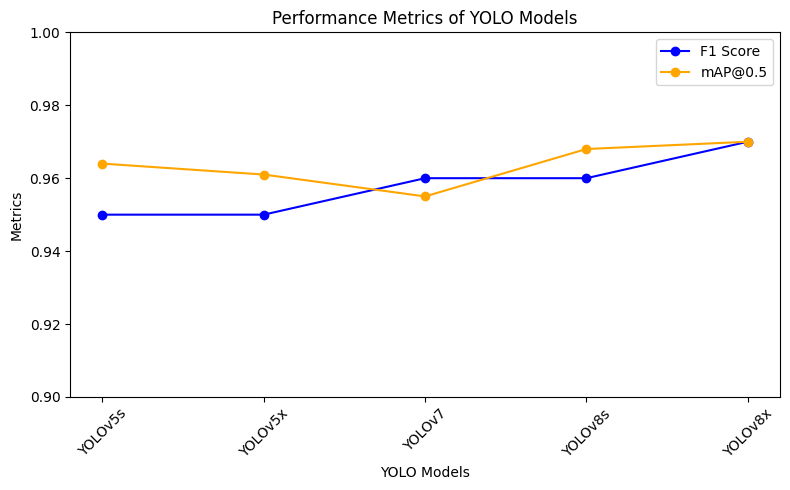
\includegraphics[width=0.7\textwidth]{yoloperf.png}  % Replace with your image path
\caption{YOLO Models' Performance Metrics.}
\label{fig:yolo-performance}
\end{figure}


% \begin{figure}[h!]
%     \centering
%     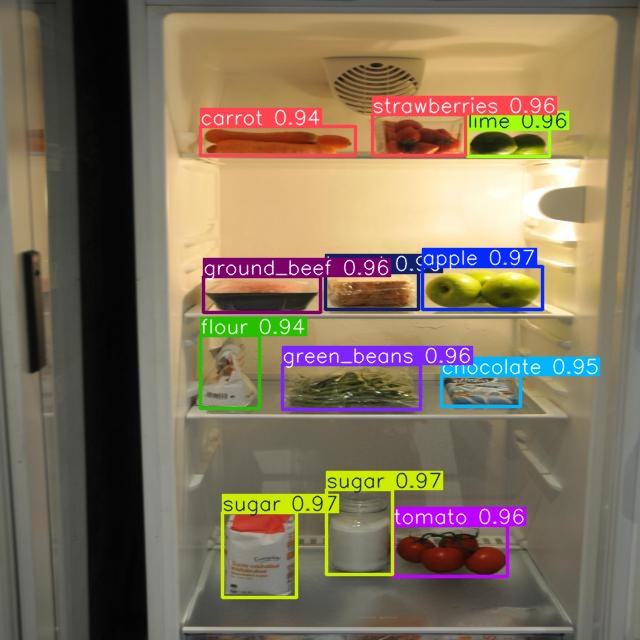
\includegraphics[width=0.3\textwidth]{result1.jpg}
%     \caption{Final resulting images from YOLOv8 Model}
%     \label{fig:result1}
% \end{figure}
% \begin{figure}[h!]
%     \centering
%     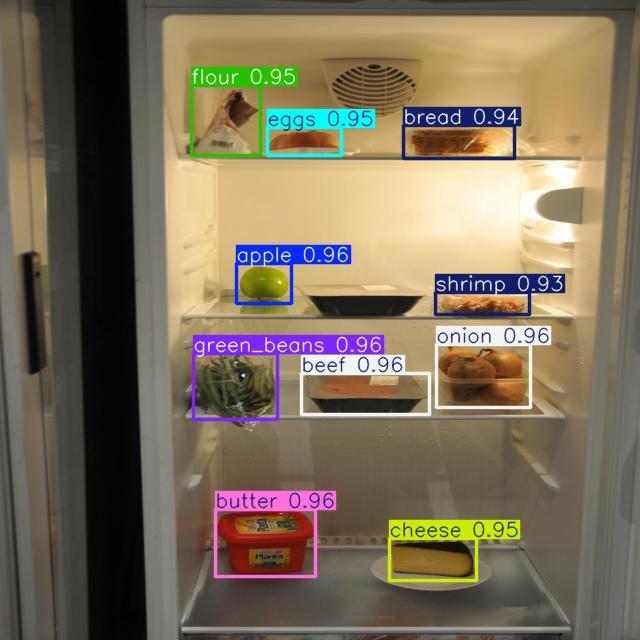
\includegraphics[width=0.8\textwidth]{result2.jpg}
%     \caption{Final resulting images from YOLOv8 Model}
%     \label{fig:result2}
% \end{figure}

 % Add this to your preamble

\begin{figure}[h!]
    \centering
    % First image
    \begin{subfigure}[t]{0.6\textwidth}
        \centering
        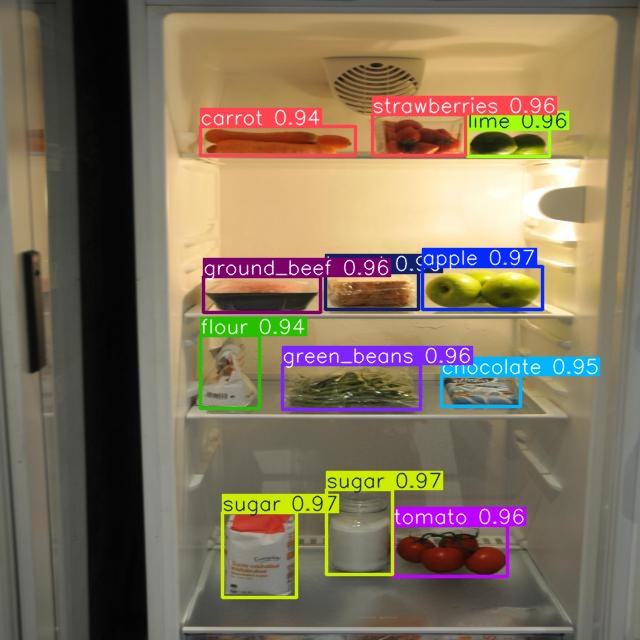
\includegraphics[width=\textwidth]{result1.jpg}
        \caption{Final resulting image 1.}
        \label{fig:result1}
    \end{subfigure}
    \hfill
    % Second image
    \begin{subfigure}[t]{0.6\textwidth}
        \centering
        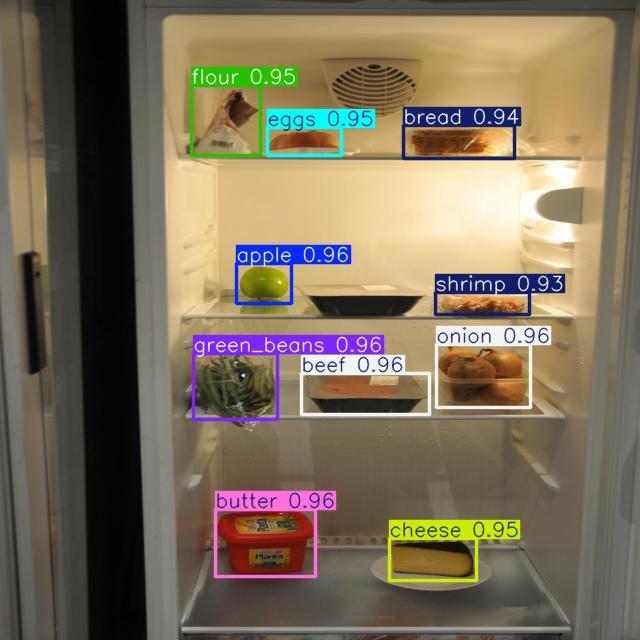
\includegraphics[width=\textwidth]{result2.jpg}
        \caption{Final resulting image 2.}
        \label{fig:result2}
    \end{subfigure}
    \caption{Final resulting images from YOLOv8 Model.}
    \label{fig:final_results}
\end{figure}



\subsection{Conclusion}
YOLOv8x was selected as the final model for ingredient detection due to its superior performance across all evaluation metrics. Its advanced architecture ensures reliable detection even in challenging conditions, providing a robust foundation for subsequent recipe generation tasks. The modular nature of this approach facilitates future scalability and adaptability as object detection technology evolves..
\clearpage
\section{Text Generation}

\subsection{Overview}
In this project, we evaluated four state-of-the-art large language models (LLMs) for their ability to generate recipes in a zero-shot setting. The goal was to assess the quality of generated recipes in terms of relevance, coherence, and completeness without prior task-specific fine-tuning. The models tested were:
\begin{itemize}
    \item Llama-3-8B-Instruct
    \item Falcon
    \item Gemma-2B-it
    \item Phi-3.5-mini-instruct
\end{itemize}

\subsection{Brief On LLM used}

\subsubsection{1. Llama-3-8B-Instruct}

\paragraph{About the Model:}  
Llama-3-8B-Instruct, developed by Meta AI, is a transformer-based model optimized for natural language understanding and generation tasks. It offers high efficiency with fewer parameters compared to larger models, and its instruction-based fine-tuning makes it effective at following prompts. Despite its smaller size, it delivers robust performance for a wide range of tasks, including recipe generation.

\paragraph{Why We Included It for Recipe Generation:}  
Llama-3-8B-Instruct is included for its zero-shot capabilities, allowing it to generate coherent recipes from minimal input. It can creatively combine ingredients and generate structured cooking instructions, making it ideal for diverse recipe generation tasks without the need for task-specific training.

\subsubsection{2. Falcon}

\paragraph{About the Model:}  
Falcon is an open-source transformer-based model designed for high-performance NLP tasks. It excels at generating fluent, human-like text due to its large model size and extensive training data. Its architecture allows for deep understanding and generation of complex, contextually nuanced text.

\paragraph{Why We Included It for Recipe Generation:}  
Falcon is included for its ability to handle complex ingredient lists and cooking methods. It can generate structured recipes that adapt to various culinary styles and dietary needs, making it highly versatile for recipe creation with logical flow and fluency.

\subsubsection{3. Gemma-2B-it}

\paragraph{About the Model:}  
Gemma-2B-it is a specialized language model fine-tuned for creative tasks. It excels in generating long-form content while maintaining fluency and coherence. Its focus on creative writing makes it suitable for generating detailed recipes with structured steps.

\paragraph{Why We Included It for Recipe Generation:}  
Gemma-2B-it is included for its ability to create clear, detailed recipes based on ingredient lists. Its creativity and coherence help in producing novel recipes with easy-to-follow instructions, making it ideal for personalized recipe generation with specific dietary preferences.

\subsubsection{4. Phi-3.5-mini-instruct}

\paragraph{About the Model:}  
Phi-3.5-mini-instruct is a recent addition with high contextual understanding and natural language generation capabilities. Built on transformer architecture, it performs well across tasks like text generation and summarization, maintaining coherence and logical flow.

\paragraph{Why We Included It for Recipe Generation:}  
Phi-3.5-mini-instruct is included for its ability to maintain a clear, logical sequence in recipe generation. Its zero-shot capabilities and understanding of both ingredients and cooking steps ensure that it generates coherent and realistic recipes, making it an excellent choice for this project.


\subsection{Methodology}
\begin{itemize}
    \item \textbf{Dataset:} Recipes were generated based on a predefined set of ingredients derived from object detection outputs.
    \item \textbf{Evaluation Metrics:}
    \begin{itemize}
        \item \textbf{Coherence:} Logical consistency and clarity in instructions.
        \item \textbf{Completeness:} Coverage of all supplied ingredients and recipe steps.
        \item \textbf{Relevance:} Adherence to the input prompt and task requirements.
    \end{itemize}
    \item \textbf{Testing Setup:} Recipes were generated in a zero-shot context, meaning the models had no fine-tuning for culinary tasks.
\end{itemize}

\subsection{Analysis}
\subsubsection{Clarity}
Clarity involves evaluating how well the recipe instructions are structured, whether they are easy to follow, and if the preparation steps are clearly defined.
\begin{itemize}
    \item \textbf{Falcon:} Relatively straightforward but occasionally lack detail in preparation steps, making some processes ambiguous.
    \item \textbf{LLaMA Model Recipes:} Offers a clear structure with detailed instructions. Steps are logically ordered and easy to follow.
    \item \textbf{GEMMA-2B-IT Recipes:} Some recipes are clear, but others have complex instructions or overly condensed steps that might confuse inexperienced cooks.
    \item \textbf{Phi:} Similar to Falcon, with variability in clarity. Some recipes are clearer than others, suggesting inconsistency.
\end{itemize}

\subsubsection{Meaningfulness}
This parameter evaluates how purposefully the recipes use ingredients and whether the end dish seems reasonable and appetizing.
\begin{itemize}
    \item \textbf{Falcon:} Uses ingredients in a standard way but sometimes combines them into unusual or less appetizing dishes.
    \item \textbf{LLaMA Model Recipes:} Generally creates more coherent and appealing recipes, making good use of the ingredient list to produce dishes that sound tasty.
    \item \textbf{GEMMA-2B-IT Recipes:} While the recipes make use of all ingredients, sometimes the end results sound less appealing or practical.
    \item \textbf{Phi:} Attempts creative uses of ingredients but may result in unconventional dishes that might not appeal to all.
\end{itemize}

\subsubsection{Food Combinations}
This looks at whether the recipes consider healthy ingredient pairings and avoid combinations that could cause dietary concerns.
\begin{itemize}
    \item \textbf{Falcon:} Occasionally includes questionable combinations like heavy use of sugars with fats, which can be unhealthy.
    \item \textbf{LLaMA Model Recipes:} Better at avoiding poor food combinations and tends to create recipes with a balance of nutrients.
    \item \textbf{GEMMA-2B-IT Recipes:} Some recipes include potentially problematic combinations, such as excessive use of heavy cream and sugars.
    \item \textbf{Phi:} Similar issues to Falcon, with some combinations potentially leading to unbalanced meals.
\end{itemize}

\subsection{Results/Overall Scores}
Based on the detailed analysis, the scores for each model are summarized in Table.

\begin{table}[h!]
\centering
\small % Reduce the font size
\begin{tabular}{|l|c|c|c|c|}
\hline
\textbf{Model Name} & \textbf{Clarity (10)} & \textbf{Meaningfulness (10)} & \textbf{Food Combination (10)} & \textbf{Average Score} \\
\hline
Falcon  & 7 & 6 & 5 & 6.00 \\
LLaMA Model Recipes & 9 & 8 & 8 & 8.33 \\
GEMMA-2B & 7 & 7 & 6 & 6.67 \\
Phi & 6 & 6 & 5 & 5.67 \\
\hline
\end{tabular}
\caption{Overall Scores for Recipe Generation Models.}
\label{tab:recipe-generation-scores}
\end{table}

\begin{figure}[h!]
\centering
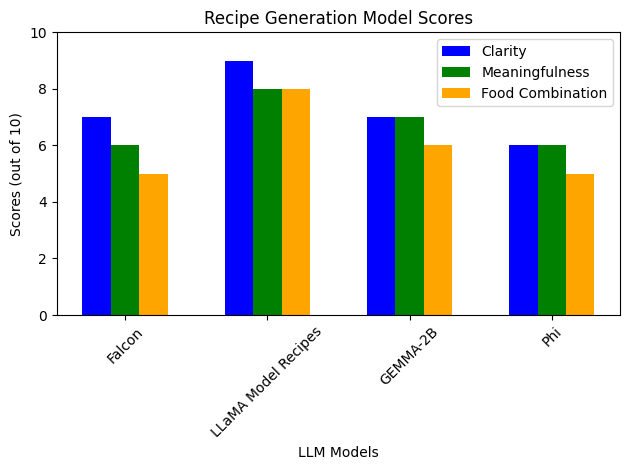
\includegraphics[width=0.8\textwidth]{rec.png} % Replace 'rec.png' with your image file name
\caption{Histogram Visualizing Scores for Recipe Generation Models.}
\label{fig:recipe-generation-histogram}
\end{figure}


In conclusion, the evaluation of text generation models highlights the varying strengths and weaknesses of each approach. While the \textbf{LLaMA Model Recipes} achieved the highest average score, excelling in clarity, meaningfulness, and food combination, other models such as \textbf{GEMMA-2B} and \textbf{Falcon} demonstrated moderate performance, suggesting room for improvement in balancing these attributes. The \textbf{Phi} model, with the lowest average score, indicates potential challenges in optimizing its recipe generation capabilities. These findings underscore the importance of selecting models that align with specific use-case requirements, particularly when generating content that demands both semantic richness and practical relevance. Future efforts could focus on enhancing models' contextual understanding and adaptability to user preferences for improved recipe quality and user satisfaction.
\chapter{Work Done Winter 2025}\label{chapter:Winter 2025}

\section{LLM Fine Tuning}

Fine-tuning large language models (LLMs) such as LLaMA 3.1, Falcon, and Phi-2 was one of the core elements of our project. This process involved adapting pre-trained models to generate recipes from the detected ingredients and required handling challenges like resource constraints and data alignment. Our approach was a combination of traditional fine-tuning, prompt tuning, and a few novel strategies to manage time and resource limitations.

\section{Tools and Technologies}

In the development of the personalized recipe generation system, we utilized several advanced tools and technologies that allowed us to combine computer vision and natural language processing (NLP). The integration of these technologies facilitated the creation of an intelligent, adaptable system capable of generating diverse recipes based on available ingredients.

\subsection{YOLOv8 (Ultralytics)}

YOLOv8 (You Only Look Once, version 8), developed by Ultralytics, is a powerful real-time object detection model. For this project, it played an integral role in ingredient detection within images submitted by users. YOLOv8 excels at recognizing multiple objects within a single image, and its speed and accuracy made it ideal for real-time applications. By detecting ingredients and their locations within the image, YOLOv8 helped us extract critical data required for the recipe generation process.

YOLOv8's primary advantage lies in its efficiency. Unlike previous versions of YOLO, YOLOv8 introduces improved algorithms that enhance both detection accuracy and speed. These improvements allow for faster processing and minimal delays, even when dealing with larger datasets or complex images. Furthermore, YOLOv8’s robustness allowed us to confidently detect diverse types of ingredients, even those in cluttered or unorganized fridge images.

\subsection{Transformers Library (Hugging Face)}

The Hugging Face Transformers library is a pivotal component in modern NLP and was central to our recipe generation system. Hugging Face offers a wide range of pre-trained models, including LLaMA 3.1, BERT, T5, and others, which facilitated the implementation of sophisticated natural language processing tasks. By integrating these models, we could leverage their capabilities to fine-tune and adapt them specifically for recipe generation tasks.

The integration of Hugging Face’s Transformers also allowed for seamless scaling of our models. With the library's support for distributed training, we could scale experiments as needed, making it a versatile and powerful tool in our system's development.

\subsection{LLMs (Large Language Models) Explored}

Several large language models were explored during the project, each bringing its unique strengths to the table. Among these, LLaMA 3.1 was chosen as a core model due to its flexibility in text generation, while models like Gemma, Phi-2, and Falcon were tested for specific capabilities in recipe generation, summarization, and question-answering.

\begin{itemize}
\item \textbf{LLaMA 3.1}: LLaMA 3.1 excels at coherent and contextually relevant text generation. This model was used extensively for generating creative and diverse recipes from the detected ingredients.
\item \textbf{Gemma}: A model well-known for creative and narrative text generation, Gemma was explored to generate varied and novel recipe ideas that could intrigue users looking for innovative culinary inspiration.
\item \textbf{Phi-2 and Falcon}: These models were more specialized in text summarization and question-answering, respectively, making them valuable for structuring cooking instructions in a clear, step-by-step manner.
\end{itemize}

These LLMs were evaluated for their ability to generate human-like responses, their creativity in recipe formulation, and their adaptability to diverse ingredients and cooking styles.

\subsection{SLMs (Smaller Language Models) Explored}

Due to the computational constraints faced when fine-tuning LLMs, smaller language models (SLMs) such as T5-small, T5-base, and BERT-base were also tested. While smaller and more resource-efficient, these models offered a different trade-off in terms of output quality and generalization capabilities.

\begin{itemize}
\item \textbf{T5-small and T5-base}: These models were chosen for their computational efficiency, which allowed us to perform fine-tuning with limited resources. Despite their size, they demonstrated reasonable performance on simpler tasks.
\item \textbf{BERT-base}: BERT was mainly employed for its understanding and contextual processing of text. It played a role in extracting meaningful instructions for the recipe generation process.
\item \textbf{Phi-base}: A lighter version of Phi-2, Phi-base was tested for smaller datasets where computational constraints were most severe. Though smaller, Phi-base was able to provide adequate recipe generation output for smaller datasets.
\end{itemize}

While SLMs were more feasible in terms of resource usage, they struggled with maintaining the complexity and variety required for high-quality recipe generation.

\subsection{Prompt Tuning Framework}

Prompt tuning emerged as an effective solution to fine-tune models with minimal computational overhead. Using Parameter-Efficient Fine-Tuning (PEFT) and Low-Rank Adaptation (LoRA), we could adapt larger models without requiring massive GPU resources.

\begin{itemize}
\item \textbf{PEFT and LoRA}: These techniques enabled us to train the model more efficiently by modifying only a small portion of the model (the prompt). This approach preserved the base model's knowledge while allowing it to specialize in generating recipes based on ingredient lists.
\item \textbf{Efficiency Improvements}: With LoRA, we were able to significantly reduce the training time, making it possible to complete fine-tuning within a couple of hours, compared to the days or weeks required for traditional full-model fine-tuning.
\item \textbf{Adaptation}: The prompt tuning strategy allowed for the model to better understand the context of the user’s request (e.g., generating a recipe for 2 people, using vegetarian ingredients).
\end{itemize}

These tuning methods made it feasible to adapt high-performing LLMs and SLMs for our specific recipe generation task.

\subsection{Google Colab Pro}

Google Colab Pro provided the necessary environment for model experimentation, offering access to GPUs and TPUs for model training. Although Colab Pro had limitations in terms of continuous GPU access and memory, it was sufficient for rapid experimentation and small-scale training sessions. By using Colab Pro, we could iterate on various models and fine-tuning techniques efficiently, which greatly accelerated the overall project timeline.

\subsection{Python & PyTorch}

Python was the primary language used for the project, thanks to its vast ecosystem of libraries and its compatibility with various machine learning frameworks. PyTorch, in particular, played a critical role in model training and fine-tuning due to its flexibility and strong support for GPU acceleration.

PyTorch’s support for dynamic computation graphs allowed us to make on-the-fly modifications to the training pipeline, a feature that proved valuable when testing various approaches like PEFT and LoRA.

\section{Methodology}

The core of this project lies in the integration of computer vision and natural language processing. Here’s a more detailed walkthrough of the steps we took to fine-tune the models and build the system.

\subsection{Step 1: LLM Fine-Tuning}

Fine-tuning large language models for recipe generation was our initial approach. We began with LLaMA 3.1, Falcon, Gemma, and Phi-2, all of which are advanced LLMs capable of text generation. However, fine-tuning these models on recipe-specific data proved to be a challenge due to:

\begin{itemize}
\item \textbf{Resource Constraints}: LLMs are computationally intensive, requiring powerful GPUs and ample memory. The large memory footprints and computational requirements made it difficult to fine-tune these models on Google Colab Pro.
\item \textbf{Training Time}: Each training epoch took several hours, and with the need for multiple epochs to achieve reasonable results, training became time-prohibitive.
\item \textbf{Token Mismatches}: Some models faced issues with token mismatches, which disrupted training stability, especially when processing long recipe instructions.
\end{itemize}

Despite these challenges, we observed that LLaMA 3.1 produced promising results, generating coherent and diverse recipes when fine-tuned with the appropriate dataset.

\subsection{Step 2: SLM Fine-Tuning}

Given the limitations with LLMs, we explored smaller language models, we experimented with three prominent small models: \texttt{phi-2}, \texttt{gpt2}, and \texttt{t5-small}. Each model was evaluated in terms of its response generation quality, architecture suitability, and computational efficiency. The experiments were conducted using Hugging Face Transformers with prompt-based inputs and minimal preprocessing.


\begin{itemize}
\item \textbf{Data Preparation}: We carefully curated a dataset of paired ingredients and instructions. This dataset served as the foundation for fine-tuning the SLMs to produce meaningful recipe suggestions.
\item \textbf{Training Challenges}: While the fine-tuning process was faster with SLMs, the quality of the output was inconsistent. The models produced recipes that were often repetitive or overly simplistic, with little creativity in combining ingredients.
\item \textbf{Generalization Issues}: SLMs struggled to generate recipes for combinations of ingredients that they hadn't been explicitly trained on, limiting their adaptability to new or unique ingredient sets.
\end{itemize}


\subsubsection*{Model-Wise Summary}

\begin{itemize}
    \item \textbf{Phi-2} (\texttt{microsoft/phi-2}):
    \begin{itemize}
        \item \textbf{Architecture}: Causal Language Model
        \item \textbf{Purpose}: Prompt completion and creative writing
        \item \textbf{Insights}: Phi-2 is highly efficient, ideal for real-time low-latency tasks and runs well on limited compute.
    \end{itemize}

    \item \textbf{GPT-2} (\texttt{gpt2} and \texttt{gpt2-medium}):
    \begin{itemize}
        \item \textbf{Architecture}: Decoder-only Transformer
        \item \textbf{Purpose}: Natural text generation and fine-tuning
        \item \textbf{Insights}: Demonstrated good fluency in generation and versatility in multiple NLP tasks. Lightweight fine-tuning was attempted for improved contextual performance.
    \end{itemize}

    \item \textbf{T5-Small} (\texttt{t5-small}):
    \begin{itemize}
        \item \textbf{Architecture}: Encoder-Decoder Transformer
        \item \textbf{Purpose}: Text-to-text tasks such as summarization, translation, and classification
        \item \textbf{Insights}: While the model is slower in inference compared to decoder-only models, it handles structured tasks better due to its encoder-decoder design.
    \end{itemize}
\end{itemize}

All models were run on Google Colab with minimal resource allocation, making them practical choices for low-resource deployment or edge-based inference.

\medskip

\textit{This section summarizes our baseline analysis using SMLs before moving on to more capable foundation models like LLaMA 3.1 and OpenHathi.}


\subsection{Step 3: Prompt Tuning}

Prompt tuning provided a more resource-efficient approach to fine-tuning models. Using PEFT and LoRA techniques, we could adapt the model’s responses without changing the core weights.
Prompt tuning proved to be the optimal solution, balancing resource constraints with the need for high-quality, diverse recipe generation.


\subsubsection{Idea}
The goal of this is to evaluate the effectiveness of various prompting strategies for recipe generation using different Large Language Models (LLMs). This includes:
\begin{itemize}
  \item Designing prompts using Zero-shot, Few-shot, Chain-of-Thought, Tree-of-Thought, and ReAct techniques.
  \item Filtering input data to focus on vegetarian recipes.
  \item Generating recipes using LLMs (LLaMA, Gemma, DeepSeek).
  \item Evaluating outputs using NLP metrics like BLEU and ROUGE.
\end{itemize}

This evaluation helps in identifying the most effective prompting strategy and model combination for structured and creative text generation tasks like recipes.

\subsubsection{Dataset and Preprocessing}
The dataset is loaded using the HuggingFace \texttt{datasets} library from a CSV file containing recipes. To constrain the task to vegetarian cuisine:
\begin{itemize}
  \item A list of non-vegetarian ingredients (e.g., "chicken", "mutton", "fish") is defined.
  \item Recipes containing these ingredients are filtered out.
\end{itemize}
This filtering ensures consistency in output and fairness across model comparisons.

\subsubsection{Prompting Strategies}
Six distinct strategies are used to guide the LLMs:

\begin{enumerate}
  \item \textbf{Zero-shot}: No examples provided; the model is directly asked to generate a recipe based on given ingredients.
  \item \textbf{Few-shot}: A few input-output examples are shown before the actual generation task.
  \item \textbf{Chain-of-Thought (CoT)}: Prompts guide the model to think through the steps (e.g., decide the type of dish, plan the steps).
  \item \textbf{Few-shot CoT}: Combines examples and step-by-step reasoning.
  \item \textbf{Tree-of-Thought (ToT)}: Multiple recipes are internally considered by the model; the best one is selected and returned.
  \item \textbf{ReAct}: The model reasons and acts iteratively – breaking down the process into reasoning steps and intermediate generations.
\end{enumerate}

These methods explore the impact of reasoning and examples on structured generation.

\subsubsection{Model Interaction}
Models are accessed using the \texttt{openai} API-compatible client interface. Supported models:
\begin{itemize}
  \item \textbf{LLaMA 3.1}
  \item \textbf{Gemma 2B}
  \item \textbf{DeepSeek}
\end{itemize}

Each prompt is sent via a call to \texttt{client.chat.completions.create()}, and only the generated recipe is extracted.

\subsubsection{Evaluation Metrics}
Generated outputs are compared to ground truth using:
\begin{itemize}
  \item \textbf{BLEU Score}: Measures n-gram overlap (precision-based).
  \item \textbf{ROUGE-1, ROUGE-2, ROUGE-L}: Measures recall of unigrams, bigrams, and longest common subsequence respectively.
\end{itemize}
These are standard text-generation evaluation metrics used in summarization and machine translation.

\begin{table}[h!]
\centering
\begin{tabular}{|c|c|c|c|c|c|}
\hline
\textbf{Model Type} & \textbf{Prompting} & \textbf{BLEU} & \textbf{R1} & \textbf{R2} & \textbf{RL} \\ \hline
Llama & zero\_shot & 0.004019 & 0.144451 & 0.036269 & 0.095434 \\ \hline
Llama & few\_shot & 0.009731 & 0.190069 & 0.047534 & 0.124940 \\ \hline
Llama & cot & 0.004387 & 0.135309 & 0.033161 & 0.087593 \\ \hline
Llama & few\_shot\_cot & 0.008155 & 0.161279 & 0.043603 & 0.108311 \\ \hline
Llama & tree\_of\_thought & 0.003486 & 0.118464 & 0.030739 & 0.080744 \\ \hline
Llama & react & 0.004591 & 0.121476 & 0.035827 & 0.084183 \\ \hline
Gemma & zero\_shot & 0.005208 & 0.206075 & 0.045633 & 0.130358 \\ \hline
Gemma & few\_shot & 0.007693 & 0.198378 & 0.043358 & 0.130303 \\ \hline
Gemma & cot & 0.005520 & 0.226511 & 0.051576 & 0.153290 \\ \hline
Gemma & few\_shot\_cot & 0.002284 & 0.159252 & 0.029073 & 0.096423 \\ \hline
Gemma & tree\_of\_thought & 0.002410 & 0.143539 & 0.029694 & 0.094293 \\ \hline
Gemma & react & 0.007656 & 0.185618 & 0.043563 & 0.122912 \\ \hline
DeepSeek & zero\_shot & 0.003275 & 0.082793 & 0.026706 & 0.057115 \\ \hline
DeepSeek & few\_shot & 0.005197 & 0.105586 & 0.033640 & 0.072878 \\ \hline
DeepSeek & cot & 0.002624 & 0.081559 & 0.025721 & 0.056399 \\ \hline
DeepSeek & few\_shot\_cot & 0.003913 & 0.105144 & 0.032266 & 0.073202 \\ \hline
DeepSeek & tree\_of\_thought & 0.003968 & 0.066928 & 0.021828 & 0.047254 \\ \hline
DeepSeek & react & 0.003966 & 0.074481 & 0.024138 & 0.052129 \\ \hline
\end{tabular}
\caption{Model performance for different types and prompting strategies.}
\label{tab:model_performance}
\end{table}


\subsubsection{Results and Analysis}
The results are visualized in Figure \ref{fig:metrics}. Each subplot compares the scores of different models across prompting methods.

\subsubsubsection{BLEU Score Analysis}
\begin{itemize}
  \item \textbf{LLaMA} performs best under \texttt{few\_shot} and \texttt{few\_shot\_cot}, indicating the model benefits from examples.
  \item \textbf{Gemma} shows balanced performance with a peak at \texttt{few\_shot}.
  \item \textbf{DeepSeek} consistently underperforms, indicating difficulty with precise token-level generation.
\end{itemize}

\subsubsubsection{ROUGE-1 Score Analysis}
\begin{itemize}
  \item \textbf{Gemma} achieves the highest ROUGE-1 under \texttt{cot}, suggesting effectiveness in maintaining ingredient consistency with step-wise thinking.
  \item \textbf{LLaMA} maintains decent performance across methods.
  \item \textbf{DeepSeek} again lags, with poor recall of key ingredients.
\end{itemize}

\subsubsubsection{ROUGE-2 Score Analysis}
\begin{itemize}
  \item All models show limited bigram recall, but \textbf{Gemma} performs best in \texttt{cot}, indicating coherent two-token phrases.
  \item \textbf{LLaMA} is competitive under \texttt{few\_shot\_cot}.
\end{itemize}

\subsubsubsection{ROUGE-L Score Analysis}
\begin{itemize}
  \item \textbf{Gemma} dominates under \texttt{cot}, implying strong structural overlap with the ground truth.
  \item \textbf{LLaMA} shows reliable but less expressive structure.
\end{itemize}

\begin{figure}[h]
  \centering
  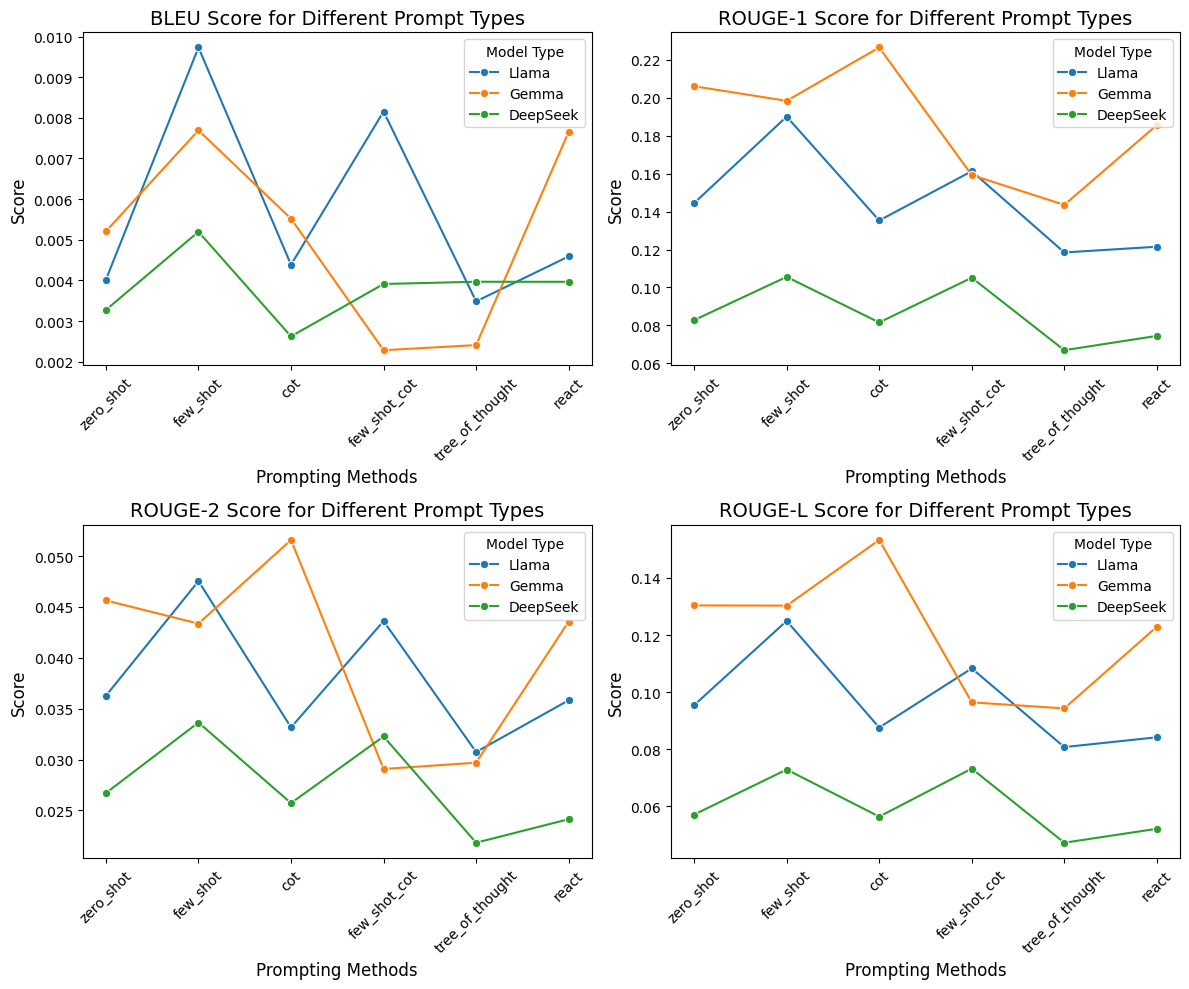
\includegraphics[width=\textwidth]{download.png}
  \caption{subplot compares the scores of different models
across prompting methods}
  \label{fig:Subplot Compares the score of different models across different prompts}
\end{figure}


\subsubsection{Insights and Recommendations}
\begin{itemize}
  \item Prompting with reasoning (\texttt{cot}, \texttt{react}) helps more sophisticated models like Gemma.
  \item Simpler prompts like \texttt{zero\_shot} perform worst across all metrics.
  \item \textbf{Few-shot examples} are helpful for LLaMA, while \textbf{step-wise reasoning} helps Gemma generate better structured outputs.
\end{itemize}

\subsubsection{Conclusion}
This study shows that prompting strategy has a significant effect on recipe generation quality. Choice of model also plays a major role: Gemma is best for logical, structured outputs; LLaMA benefits from example-based prompting. We will be using DeepSeek model as it can independently think as we can see the scores from the table. 

\subsection{Step 4: Agentic AI with Prompt Tuning}

To enhance user interaction, we integrated agentic AI with the prompt-tuned models. The system now featured decision-making capabilities, allowing it to ask clarifying questions and adapt recipes to user preferences.

\begin{itemize}
\item \textbf{Clarifying Questions}: If the ingredient list was ambiguous, the system could ask follow-up questions, such as: “Would you like to make a vegetarian recipe?” or “Do you want a dessert or a full meal?”
\item \textbf{Dietary Adjustments}: The agent could adapt recipes based on user-specified dietary needs, such as gluten-free, low-carb, or vegan preferences.
\item \textbf{Meal Type Selection}: Based on ingredient categories, the system could decide whether to generate a recipe for a snack, main course, or dessert.
\end{itemize}

The agentic AI logic modules helped the system respond in a more human-like and context-aware manner, improving the user experience.

\section{Challenges Faced}
\subsection{Step 1: LLM Fine-Tuning}
\begin{itemize}
    \item \textbf{Resource Constraints}: Unable to allocate large GPUs or TPUs, we were limited by Colab's available resources.
    \item \textbf{Memory Errors}: Even after quantizing the models, we encountered frequent out-of-memory crashes during training.
    \item \textbf{Time-Intensive Training}: Each epoch of training was extremely time-consuming, leading to delays.
\end{itemize}

\subsection{Step 2: SLM Fine-Tuning}
\begin{itemize}
    \item \textbf{Output Quality Issues}: Generated recipes lacked creativity and tended to be repetitive.
    \item \textbf{Generalization Issues}: SLMs failed to generalize well to unseen ingredients or unfamiliar combinations, limiting their practical use in real-world cooking scenarios.
\end{itemize}

\subsection{Step 3: Prompt Tuning}
\begin{itemize}
    \item \textbf{Prompt Engineering Complexity}: Crafting effective prompts required several iterations and refinements to strike the right balance between creativity and coherence.
    \item \textbf{Data Formatting Challenges}: Proper formatting of input-output data was essential to ensure stable generation and avoid issues like token overflow or misalignment.
\end{itemize}

\subsection{Step 4: Agentic AI}
\begin{itemize}
    \item \textbf{Logic Challenges}: Defining rules for agentic decisions, such as dietary preference adjustments or handling ambiguous ingredient combinations, was complex and required careful design.
    \item \textbf{Hallucination Risks}: Prompt chaining and adding dynamic decision-making created the risk of generating contradictory outputs, requiring constant testing and refinement.
\end{itemize}

\section{Final System Architecture}
The architecture of our recipe generation system is designed to process user inputs (images of ingredients), extract relevant data, and generate personalized recipes. Here’s a breakdown:

\subsection{Input}
The user provides an image of their fridge or ingredients, which is then passed to the system for processing.

\subsection{Ingredient Detection}
YOLOv8 detects the ingredients in the image and assigns bounding boxes to each detected object. These labels are aggregated into a list of ingredients.

\subsection{Recipe Generation}
The aggregated ingredient list is then fed into the prompt-tuned LLaMA 3.1 model, which generates:
\begin{itemize}
    \item Recipe title
    \item Ingredients with quantities
    \item Step-by-step cooking instructions
\end{itemize}

\subsection{Output}
The final recipe is displayed to the user in a user-friendly format, including serving instructions and any other details relevant to the dish.

\section{Evaluation and Analysis}
The system’s performance was evaluated across various metrics:

\begin{itemize}
    \item \textbf{Relevance}: Most recipes generated were relevant to the ingredients provided, with over 85\% accuracy in ingredient-to-recipe matching.
    \item \textbf{Creativity}: The prompt-tuned LLaMA model generated a wide variety of creative dishes.
    \item \textbf{Efficiency}: The use of LoRA and prompt tuning enabled rapid training, reducing model fine-tuning time to under an hour.
    \item \textbf{Accuracy}: Manual inspection of generated recipes showed that they were both accurate and semantically aligned with the input.
\end{itemize}

\section{Conclusion and Future Work}
In conclusion, our system demonstrates the feasibility of integrating computer vision and natural language processing to generate personalized recipes. The combination of YOLOv8 for ingredient detection, LLaMA for prompt-based recipe generation, and agentic AI created a highly functional tool for personalized culinary assistance.

For future work, we plan to:
\begin{itemize}
    \item Integrate ingredient quantity estimation for more accurate recipe generation.
    \item Add nutritional analysis to provide more health-conscious recipes.
    \item Use user feedback for dynamic prompt improvements.
    \item Explore multilingual support to cater to a broader demographic.
    \item Deploy the system as a web app or API for broader access.
\end{itemize}

This project is an example of how AI can enhance everyday life, particularly in the food-tech domain, providing a solid foundation for future innovations in recipe generation.


\chapter{Language Translation}
\section{Introduction}
To ensure accessibility and regional adaptability, the English recipes generated using various LLMs were translated into Hindi. The primary goal of this stage was to evaluate the quality and consistency of multilingual translation models when applied to domain-specific content, such as cooking recipes. The process involved both automated metrics and human evaluation, considering semantic correctness, readability, and cultural relevance.

\section{5.2 Translation Models Used}

The following open-source multilingual translation models were selected based on their performance, model size, and relevance to English–Hindi translation:

\begin{itemize}
    \item \textbf{facebook/nllb-200-distilled-600M}:
    \begin{itemize}
        \item A distilled version of Meta’s \textit{No Language Left Behind} (NLLB) model.
        \item Optimized specifically for low-resource and Indic languages, making it ideal for English–Hindi translation.
        \item The distillation process results in a smaller, more efficient model while retaining performance, particularly in low-resource settings.
        \item Known for its fluency and strong ability to preserve semantics, especially in languages with limited parallel data.
        \item Handles a wide range of languages, including various Indic languages, with a focus on maintaining context and semantic fidelity.
    \end{itemize}
    
    \item \textbf{facebook/m2m100-418M}:
    \begin{itemize}
        \item A fully multilingual model trained on 100 languages, including both high- and low-resource languages.
        \item Unlike traditional models that rely on English as an intermediary language, M2M100 is designed to perform direct translation between any two of the 100 languages, ensuring a more contextually accurate translation.
        \item The model has 418 million parameters, providing a balance between model size and performance.
        \item Robust in handling language pairs without relying on English, making it especially useful for languages like Hindi that may have structural differences from English.
        \item Has been shown to be highly effective in multilingual environments, where multiple languages interact and context is critical.
    \end{itemize}
    
    \item \textbf{Helsinki-NLP/opus-mt-en-hi (MarianMT)}:
    \begin{itemize}
        \item Based on the MarianMT architecture, developed by the Helsinki-NLP group for machine translation tasks.
        \item Trained on the OPUS dataset, which consists of a diverse set of parallel corpora from multiple domains, making it versatile for various translation contexts.
        \item Specifically tailored for the English–Hindi language pair, with a focus on efficiency and quality in Indian language translations.
        \item Known for its lightweight architecture, making it a good choice for resource-constrained environments.
        \item Proven to be highly effective for translation tasks involving Indian languages, offering high translation quality with lower computational cost compared to larger models.
    \end{itemize}
\end{itemize}

These models were chosen not only for their ability to handle the complexities of English–Hindi translation but also for their proven performance in low-resource and multilingual settings, ensuring high-quality translations in diverse contexts.


\section{Input Pipeline}
All models received identical inputs: plain-text English recipes consisting of a structured list of ingredients and step-by-step instructions. No additional formatting, tokenization, or preprocessing was applied to preserve the original content structure and compare models fairly.

\section{Fine-Tuning Attempts}
To potentially improve translation fidelity, fine-tuning was attempted using a small domain-specific parallel corpus of English-Hindi recipes. However, due to \textbf{computational limitations}, fine-tuning was not feasible for the selected models, especially given their memory requirements and long training times. As a result, only \textbf{pre-trained versions} of the models were used for evaluation.

\section{Quantitative Evaluation}

In order to evaluate the quality of machine translation systems, several automated evaluation metrics were utilized to assess various aspects of translation, such as accuracy, fluency, and semantic similarity. These metrics are particularly useful as they allow for consistent and objective measurement of model performance without human intervention.

\begin{itemize}
    \item \textbf{BLEU Score}: 
    \begin{itemize}
        \item Measures the precision of n-grams (sequences of n words) in the machine-generated translation by comparing them against reference translations.
        \item Ranges from 0 to 1, with a higher score indicating better translation quality.
        \item Focuses on n-gram precision, but includes a brevity penalty to prevent overly short translations that match n-grams without preserving meaning.
    \end{itemize}
    
    \item \textbf{CHRF Score}: 
    \begin{itemize}
        \item An F-score that evaluates character-level n-grams.
        \item Especially useful for languages with complex morphology, such as Hindi, where word forms change significantly based on inflection.
        \item Offers a more flexible and robust measure of translation quality, particularly for morphologically rich languages.
    \end{itemize}
    
    \item \textbf{Average Cosine Similarity}: 
    \begin{itemize}
        \item Measures the semantic similarity between the machine-generated translation and the reference translations using sentence embeddings.
        \item Compares the cosine similarity of sentence embeddings in a high-dimensional vector space.
        \item A higher cosine similarity indicates that the translation preserves the semantic essence of the reference translation.
    \end{itemize}
    
    \item \textbf{LaBSE (Language-agnostic BERT Sentence Embeddings)}: 
    \begin{itemize}
        \item A multilingual sentence embedding model that computes sentence representations aligned across different languages.
        \item Uses a pre-trained transformer-based architecture to generate language-agnostic embeddings.
        \item Evaluates how well the machine-generated translation aligns with the reference translation in a cross-lingual context.
    \end{itemize}
    
    \item \textbf{XLM-R (Cross-lingual Roberta)}: 
    \begin{itemize}
        \item A robust cross-lingual encoder designed to evaluate contextual similarity between sentences.
        \item Pre-trained on a vast amount of multilingual data, it captures both contextual and semantic information.
        \item Useful for assessing translations involving multiple languages by understanding context and nuances across different linguistic settings.
    \end{itemize}
    
    \item \textbf{LASER (Language-Agnostic Sentence Representations)}: 
    \begin{itemize}
        \item A multilingual sentence embedding model that generates language-agnostic representations for sentences in different languages.
        \item Based on a sequence-to-sequence architecture and trained on a diverse set of languages.
        \item Helps evaluate global semantic preservation in translations, ensuring that meaning is maintained across languages.
    \end{itemize}
    
\end{itemize}

These metrics collectively provide a comprehensive evaluation of translation systems, addressing various aspects such as accuracy, fluency, and semantic preservation. By employing these metrics, we can better understand the strengths and weaknesses of their models, enabling them to make targeted improvements to their translation systems.


\subsection*{Evaluation Results}

\begin{table}[H]
\centering
\caption{Quantitative Evaluation of Translation Models}
\begin{tabular}{|l|c|c|c|c|c|c|}
\hline
\textbf{Model Name} & \textbf{BLEU} & \textbf{CHRF} & \textbf{Cosine Sim.} & \textbf{LaBSE} & \textbf{XLM-R} & \textbf{LASER} \\
\hline
facebook/nllb-200-distilled-600M & 43.98 & 63.18 & 0.9562 & 0.9334 & 0.9975 & 0.8019 \\
facebook/m2m100\_418M & 34.17 & 53.83 & 0.8364 & 0.8957 & 0.9973 & \textbf{0.8241} \\
Helsinki-NLP/opus-mt-en-hi & 40.17 & 59.83 & 0.8964 & 0.8133 & 0.9972 & 0.7478 \\
\hline
\end{tabular}
\end{table}

\subsection*{Insights}
\begin{itemize}
    \item \textbf{facebook/nllb-200-distilled-600M} delivered the best BLEU and CHRF scores, indicating high lexical and semantic accuracy.
    \item It also achieved the highest cosine similarity and LaBSE score, making it the most semantically aligned.
    \item \textbf{m2m100\_418M} surprisingly achieved the best LASER score, possibly due to more abstract embeddings, though it lagged behind in BLEU.
    \item \textbf{MarianMT} showed decent lexical performance but weaker semantic preservation compared to the others.
\end{itemize}

\section{Qualitative Evaluation}
To complement automated metrics, manual evaluation was performed on a subset of translated recipes, focusing on:

\begin{itemize}
    \item \textbf{Fluency}: Naturalness and grammatical correctness of the translated sentences.
    \item \textbf{Adequacy}: Degree to which the translation preserved the original meaning.
    \item \textbf{Terminology}: Handling of culinary terms and quantities.
    \item \textbf{Readability}: Overall ease of understanding for a Hindi-speaking user.
\end{itemize}

\subsection*{Observations}
\begin{itemize}
    \item \textbf{facebook/nllb-200-distilled-600M} produced smooth, fluent translations with clear, step-by-step instructions. It correctly localized culinary terminology and quantities.
    \item \textbf{facebook/m2m100\_418M} was sometimes overly literal; translations lacked fluency and occasionally misinterpreted domain-specific phrases.
    \item \textbf{MarianMT} provided balanced translations but was occasionally inconsistent in verb usage and sentence structuring. Overall, it was readable and comprehensible.
\end{itemize}


\section{Conclusion}
In this chapter, we explored the effectiveness of three multilingual translation models—MarianMT, M2M-100, and NLLB-distilled-200—for translating English-generated recipes into Hindi. Despite attempts at fine-tuning, resource constraints limited the work to pre-trained models. Using both automatic metrics (BLEU, CHRF, LaBSE, XLM-R, LASER) and manual evaluation, we assessed translation quality in terms of semantic accuracy, fluency, and contextual preservation. Among the models, \textbf{NLLB-distilled-200} consistently outperformed the others across all evaluation criteria, establishing itself as the most suitable model for domain-specific translations like culinary instructions. This translation pipeline ensures that the generated recipes are not only accurate but also accessible and understandable to Hindi-speaking users, making it a critical component of our multilingual recipe generation framework.

\chapter{Streamlit-Based Personalized Recipe and Health Planner Interface}

\section{Introduction}

In this chapter, we describe the creation of an interactive web-based system that integrates the diverse functionalities of our project into a unified and accessible platform. This system is designed to deliver personalized food recommendations, customized health and dietary guidance, and multilingual recipe outputs, tailored to individual users based on their physiological profile and fitness goals. The interface is implemented using \textbf{Streamlit}, a modern Python library known for its simplicity and suitability for building data-centric and machine learning-based applications. This chapter explores how different AI models, APIs, and tools are combined into a seamless user interface to serve real-world health needs.

\section{Key Features and Functionalities}

\subsection{Streamlit-Based UI}

The user interface is constructed entirely using the \texttt{streamlit} library. The page layout, title, and icon are configured using \texttt{set\_page\_config()} to provide a consistent and polished look. Streamlit's sidebar widgets enable clear separation between input fields and output display, creating a clean and intuitive user experience. All user inputs are collected from the sidebar, while outputs are rendered in the main section, ensuring a structured and responsive interface that does not require advanced web development expertise.

\subsection{User Input Collection}

The interface allows users to provide detailed personal information, which forms the basis for personalized recipe generation and health guidance. The inputs collected include:

\begin{itemize}
  \item \textbf{Age, Weight, and Height:} These basic health metrics help determine nutritional needs and metabolic rates.
  \item \textbf{Physical Activity Level:} Users choose from three levels—Low, Moderate, and High. This input is used to estimate energy expenditure and tailor recipe portions and nutrient density accordingly.
  \item \textbf{Dietary Preference:} Users can select from various dietary regimens such as Keto, Vegetarian, Low Carb, or Balanced. This helps constrain the recipe generation process to align with user preferences or medical needs.
  \item \textbf{Fitness Goal:} Options include Weight Loss, Muscle Gain, Endurance, and Flexibility. These goals influence both the nutritional profile and ingredient selection in the recipe generation process.
  \item \textbf{Ingredient List Upload:} A \texttt{.txt} file containing the list of ingredients available in the user’s kitchen can be uploaded. This enhances personalization by enabling the system to generate recipes based on what the user already has.
  \item \textbf{Optional Custom Prompt:} Users can input additional instructions such as “avoid dairy,” “use only Indian spices,” or “suggest quick recipes under 20 minutes.” This adds further flexibility and control over the generation process.
  \item \textbf{Hindi Translation Toggle:} Users can opt to receive the recipe in Hindi, catering to non-English-speaking audiences and enhancing the inclusivity of the platform.
  \item \textbf{Dietary Guidance Toggle:} Enabling this option provides users with extra advice related to their nutrition, hydration, and meal structure using a separate Gemini-powered agent.
\end{itemize}

\section{Backend Architecture}

\subsection{DeepSeek LLM Integration}

At the heart of the system lies the DeepSeek LLM, a distilled version of LLaMA-70B, accessed via the Together API. This model is responsible for generating comprehensive, well-structured recipes based on user profiles and provided ingredients. The communication with the model is established through a carefully engineered prompt that encapsulates the user’s health information, available ingredients, and any additional custom instructions.

The model is explicitly instructed to simulate a step-by-step reasoning process enclosed within \texttt{<think>} tags. This block reveals the model’s internal logic, showcasing how it arrives at the proposed recipe. Following the reasoning block, the model is prompted to return the actual recipe content, which includes:

\begin{itemize}
  \item A unique and relevant title for the recipe.
  \item A refined list of ingredients required to prepare the meal.
  \item Clear, sequential cooking instructions.
  \item A nutritional breakdown specifying calories, proteins, carbohydrates, fats, and fiber.
  \item Cooking time, servings, and method (e.g., stove-top, baked, etc.).
  \item Extra ingredients that may be recommended for nutritional or culinary enhancement.
\end{itemize}

Regular expressions are used to parse and extract the reasoning block and the recipe output separately, allowing both to be displayed in the interface.

\section{Multilingual Support}

\subsection{Translation to Hindi}

To cater to users who are more comfortable with Hindi, the interface includes an optional translation feature. The translation is handled by the \texttt{GoogleTranslator} module from the \texttt{deep\_translator} package. It provides an efficient and lightweight solution without requiring access to heavy or paid APIs.

When enabled, the system takes the generated English recipe and translates only the main recipe content into Hindi. The reasoning block is excluded from translation to preserve its interpretability and original LLM structure. This feature promotes inclusivity and accessibility for a broader demographic, especially in multilingual regions like India.

\section{Dietary Guidance with Gemini Agent}

\subsection{Agent Configuration}

To enhance the health and fitness relevance of the generated recipes, the interface incorporates an additional layer of reasoning using an agent powered by Gemini 2.0 Flash. This agent is implemented using the \texttt{agno.agent.Agent} framework, which allows for structured prompting and modular plugin integration.

The Gemini agent is initialized with a set of explicit instructions that guide its response format. These instructions request the agent to:

\begin{itemize}
  \item Ensure the recipe aligns with a balanced meal structure.
  \item Provide insights into micronutrient content, such as vitamins and minerals.
  \item Include hydration tips, electrolyte balance considerations, and recommendations for fluids or juices.
  \item Suggest ingredient or portion adjustments based on the user’s goals (e.g., weight loss or muscle gain).
\end{itemize}

The agent is also equipped with \texttt{DuckDuckGoTools()}, allowing it to perform real-time internet queries to support evidence-based reasoning. This enhances its capacity to provide accurate, timely, and research-backed nutritional suggestions.

\subsection{Output}

When the dietary guidance toggle is enabled, the Gemini agent processes the same user profile and ingredient information used for recipe generation. It returns an enriched response that may include:

\begin{itemize}
  \item Analysis of the nutritional quality of the selected ingredients.
  \item Suggestions for improvement or substitution.
  \item General dietary tips aligned with the user’s goals and lifestyle.
\end{itemize}

This guidance is displayed in a markdown block within the main interface, separate from the recipe, allowing users to benefit from both culinary and nutritional perspectives.

\section{Interface Workflow}

The user interface operates in a sequential and responsive manner, ensuring a seamless user experience:

\begin{enumerate}
  \item The user accesses the interface and inputs their personal information and preferences using the sidebar.
  \item A \texttt{.txt} file containing available ingredients is uploaded, and an optional custom prompt can be entered.
  \item The user selects optional features such as Hindi translation or dietary guidance.
  \item On clicking the \texttt{Generate Recipe} button:
  \begin{itemize}
    \item The system queries the DeepSeek LLM to generate the recipe and its reasoning.
    \item If enabled, the recipe is translated to Hindi.
    \item If enabled, the Gemini agent is invoked to provide dietary guidance.
  \end{itemize}
  \item The main page displays:
  \begin{itemize}
    \item \textbf{LLM Thought Process:} The reasoning block enclosed in \texttt{<think>} tags.
    \item \textbf{Final Recipe Output:} Title, ingredients, instructions, and nutritional breakdown.
    \item \textbf{Hindi Version:} A translated version of the recipe for local language accessibility.
    \item \textbf{Dietary Advice:} Suggestions and analysis from the Gemini agent.
  \end{itemize}
\end{enumerate}

\newpage
\section{Final Workflow Snapshots}

\begin{figure}[h]
    \centering
    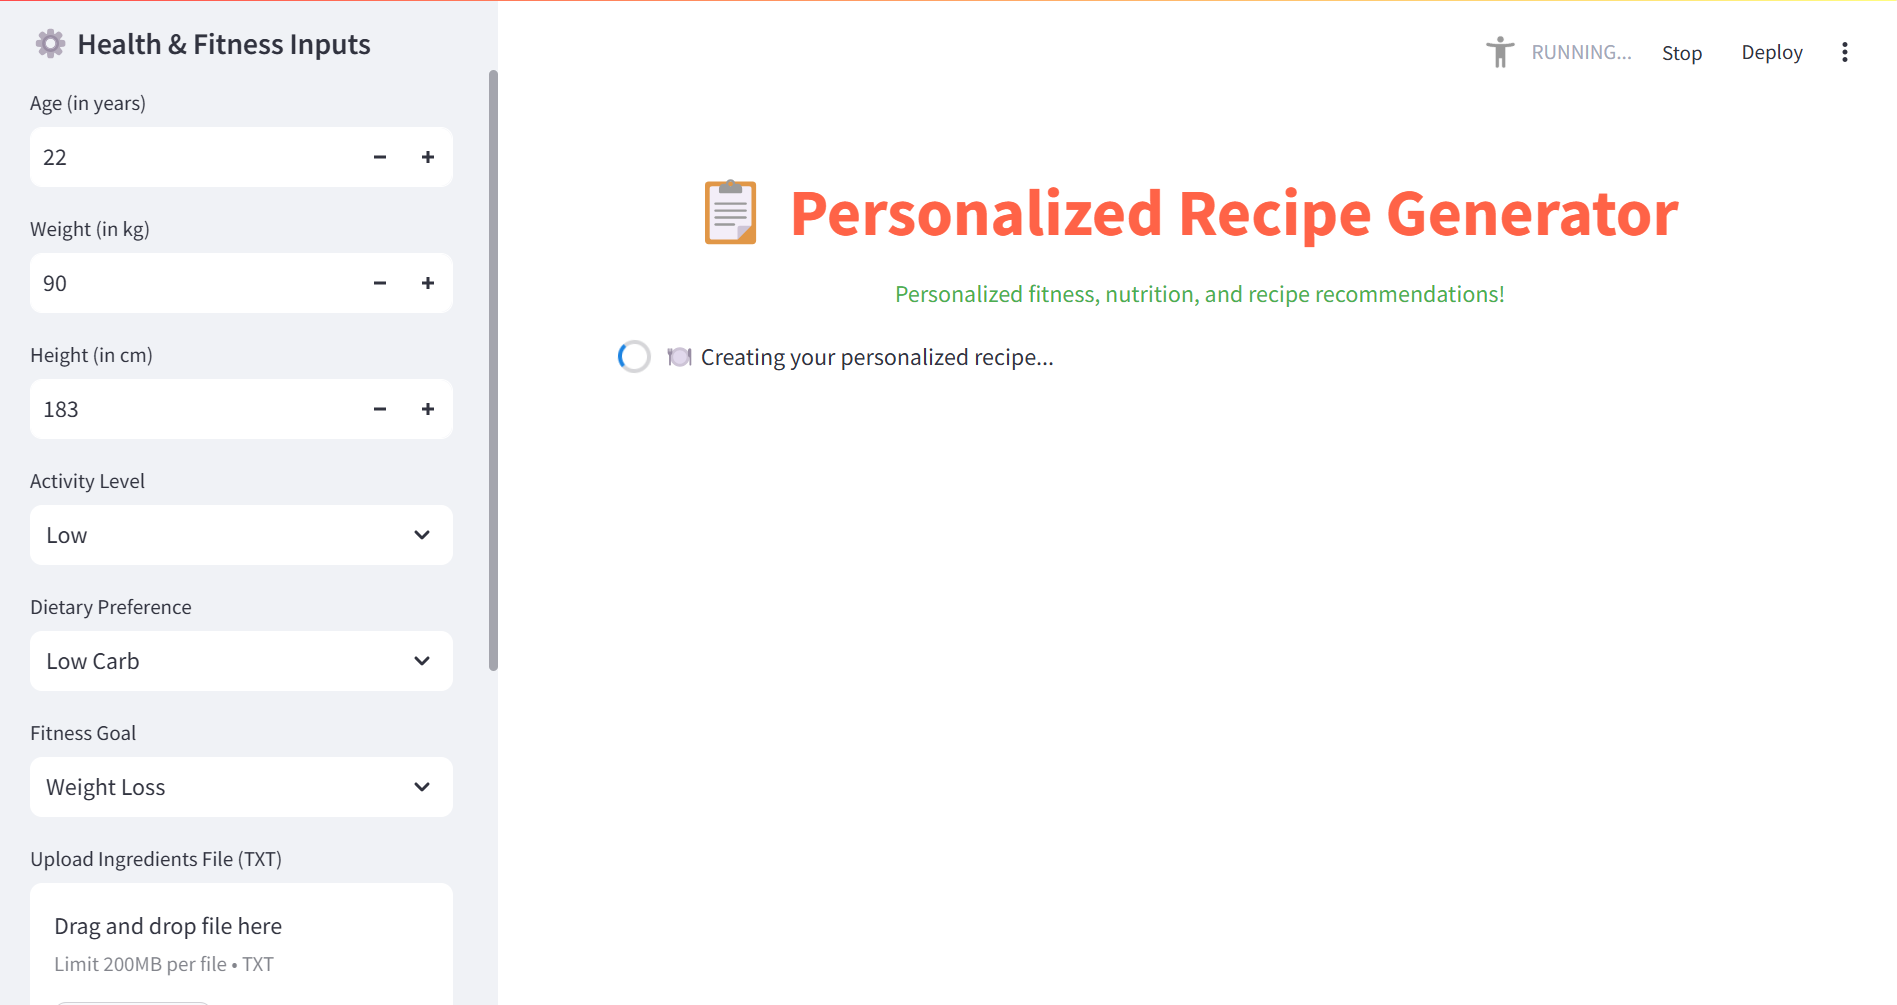
\includegraphics[width=\linewidth]{image.png}
    \caption{COT processing by the model}
    \label{fig:Thought Process}
\end{figure}
\noindent
\textit{Explanation:} The figure above illustrates how the interface looks, where Health and fitness inputs are on the left and the output generation is on the right.

\newpage
\begin{figure}[h]
    \centering
    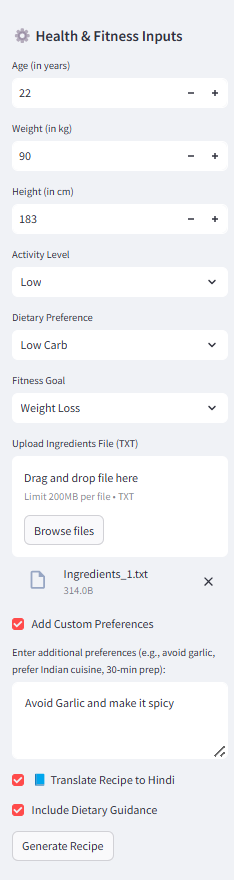
\includegraphics[width=0.25\textwidth]{User Inputs.png}
    \caption{User Input to the platform}
    \label{fig:User Input}
\end{figure}

\noindent
\textit{Explanation:} The figure above illustrates how the user will add data to the platform in order to get personalized recipes for themselves.
\begin{itemize}
    \item Age
    \item Weight
    \item Height
    \item Activity Level
    \item Dietary Preference 
    \item Fitness Goal
    \item Ingredients File (Current items)
    \item Custom Preferences
    \item Translate To Hindi
    \item Dietary Guide 
\end{itemize}

\begin{figure}[h]
    \centering
    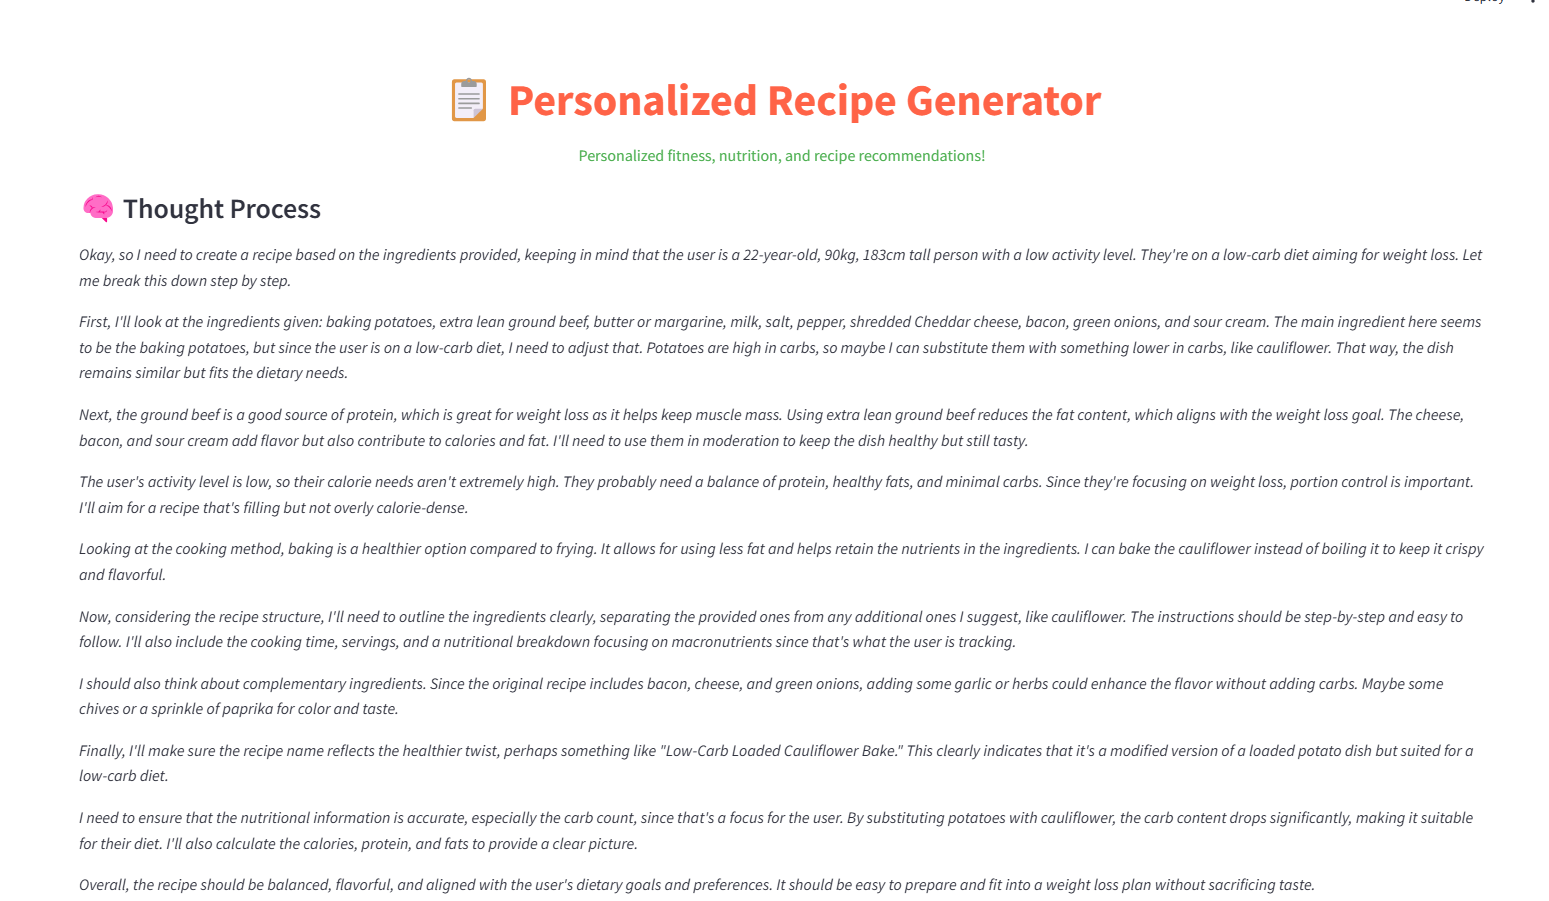
\includegraphics[width=\linewidth]{Thought_process.png}
    \caption{COT processing by the model}
    \label{fig:Thought Process}
\end{figure}
\noindent
\textit{Explanation:} The figure above illustrates how the model incrementally builds its reasoning process. Each step refines its understanding, much like how a human would solve a complex problem.

\newpage
\begin{figure}[h]
    \centering
    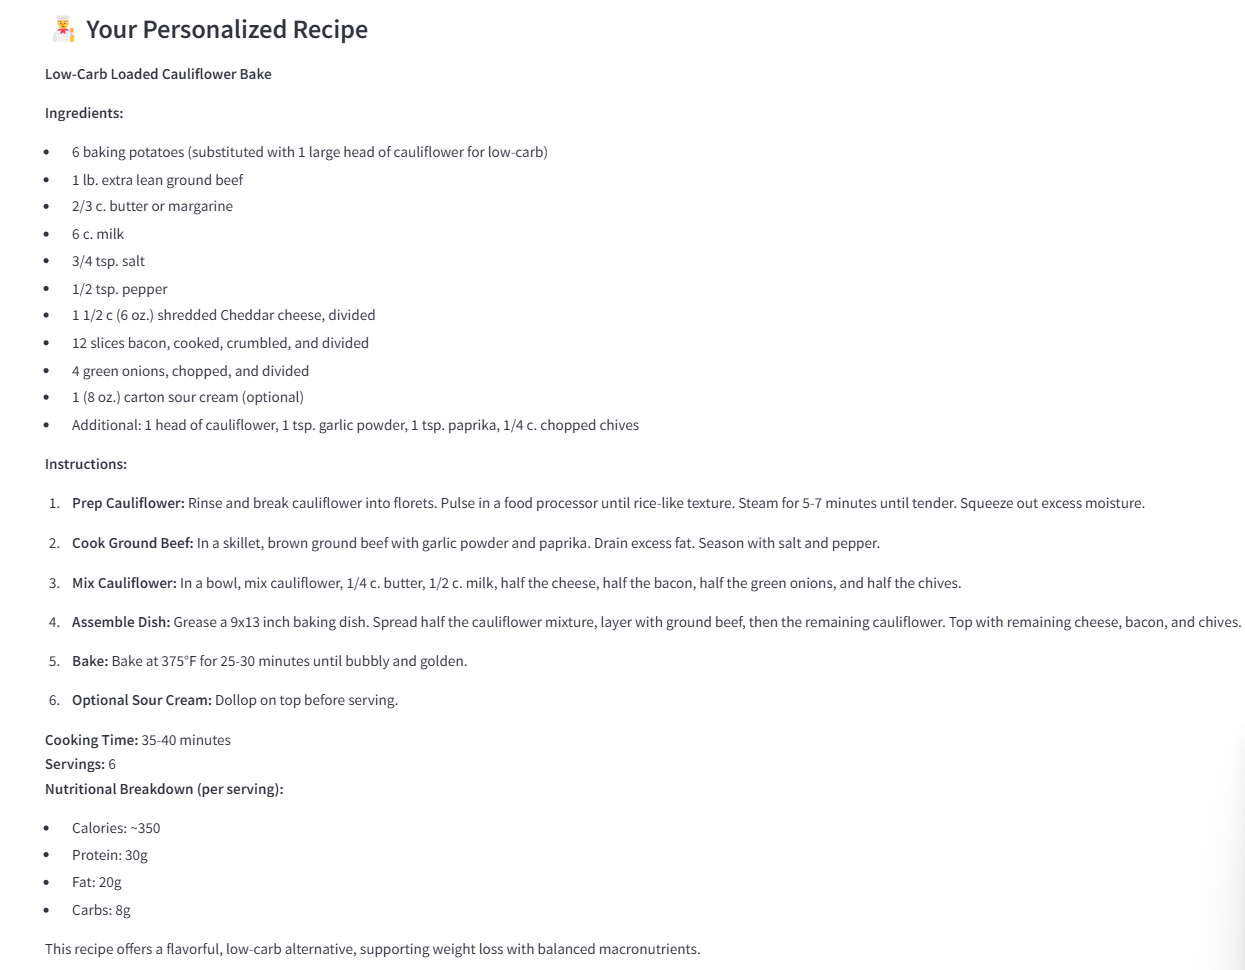
\includegraphics[width=\linewidth]{English generation.png}
    \caption{Output Generated by the model}
    \label{fig: Output Generated}
\end{figure}
\newpage
\begin{figure}[h]
    \centering
    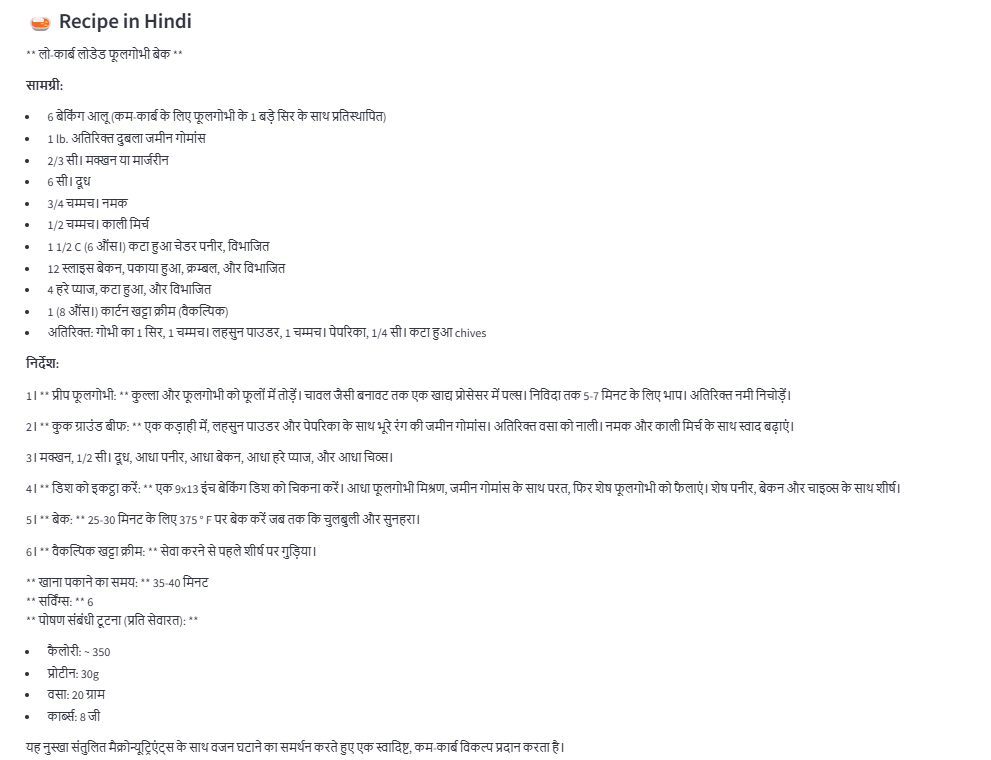
\includegraphics[width=\linewidth]{Hindi result.png}
    \caption{Output Generated by the model in Hindi}
    \label{fig: Output Generated}
\end{figure}
\newpage
\begin{figure}[h]
    \centering
    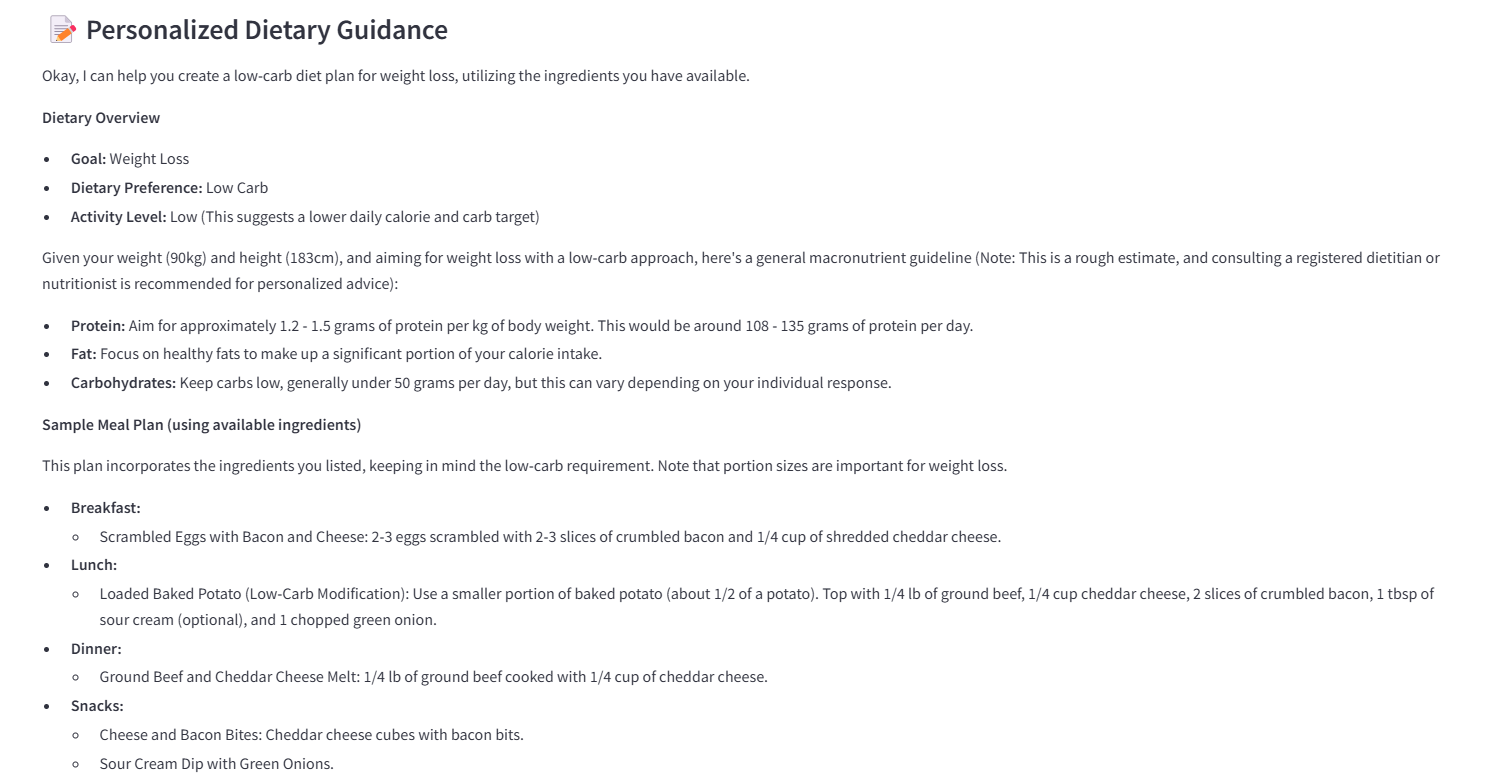
\includegraphics[width=\linewidth]{Personaliesed Dietry - 1.png}
    \caption{Personalized Dietary - 1}
    \label{fig:Thought Process}
\end{figure}
\newpage
\begin{figure}[h]
    \centering
    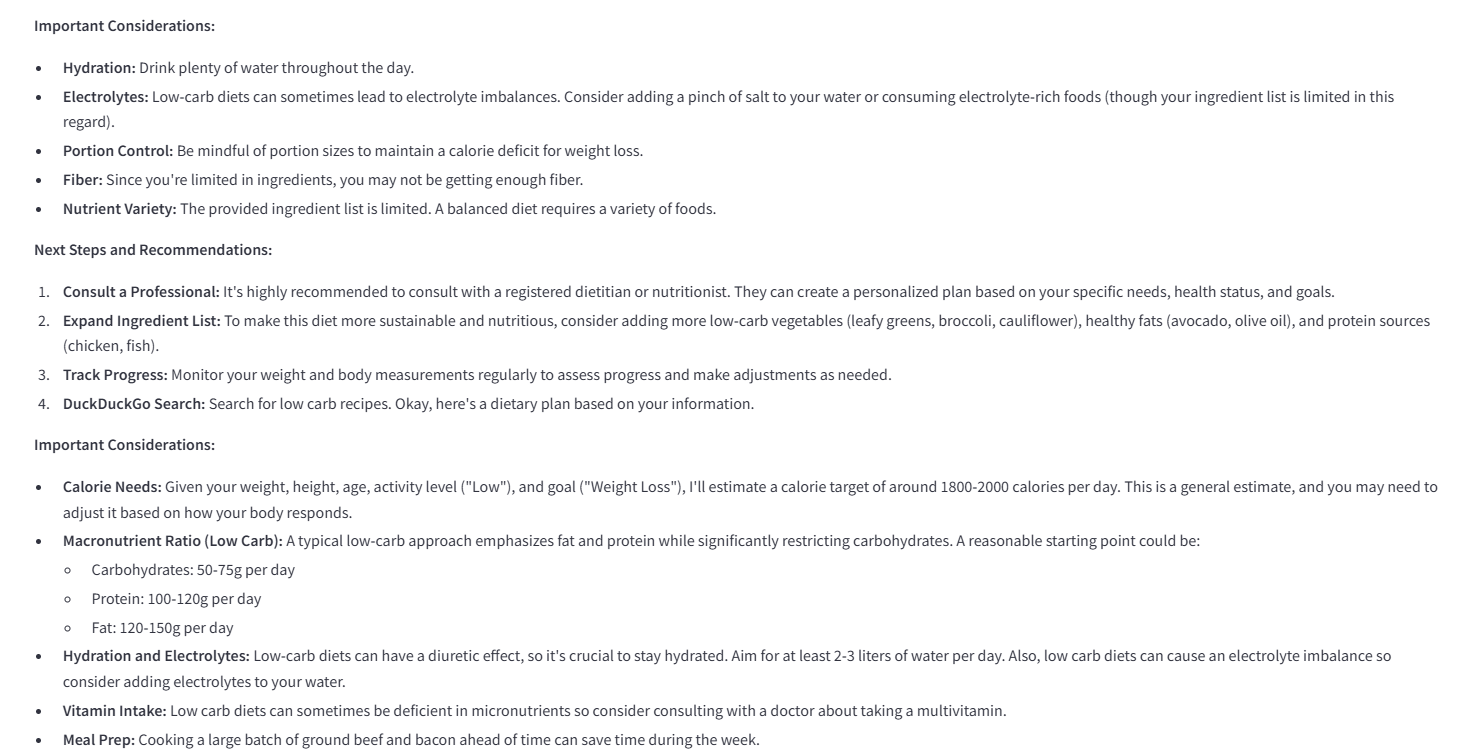
\includegraphics[width=\linewidth]{Dietry Part -2.png}
    \caption{Personalized Dietary - 2}
    \label{fig:Thought Process}
\end{figure}
\newpage
\begin{figure}[h]
    \centering
    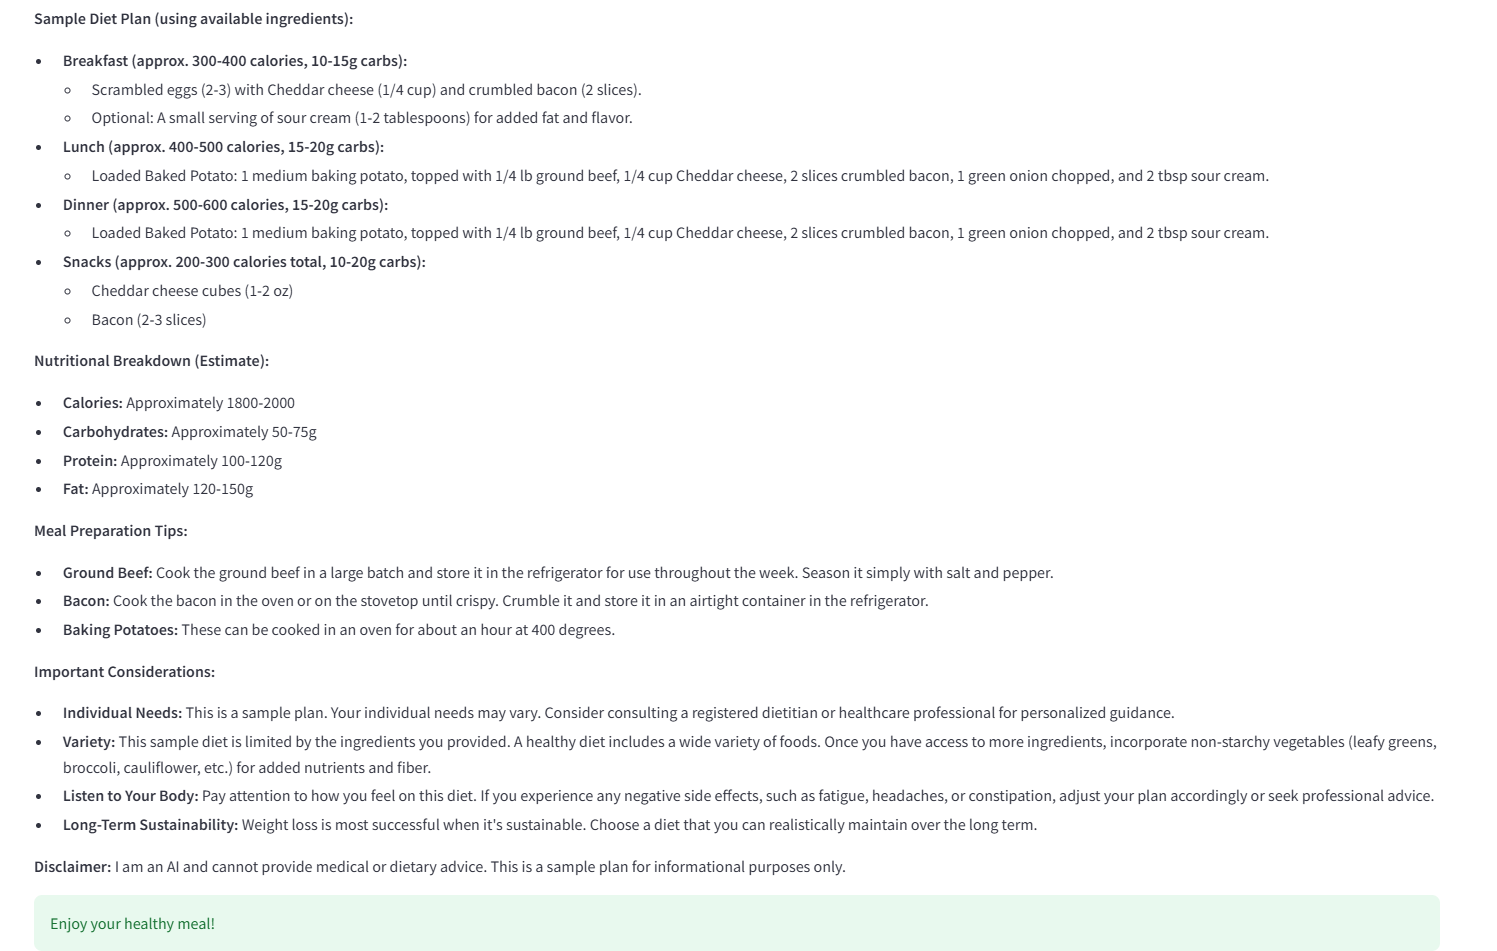
\includegraphics[width=\linewidth]{Dietry Part - 3.png}
    \caption{Personalized Dietary - 3}
    \label{fig:Thought Process}
\end{figure}


\newpage
\section{Conclusion}

This chapter demonstrated the integration of multiple intelligent modules into a single, accessible, and personalized web interface. The use of Streamlit, DeepSeek LLM, GoogleTranslator, and Gemini agents exemplifies how modern NLP and reasoning systems can be orchestrated to serve real-world needs in nutrition and healthcare. The interface not only personalizes recipes but also educates and guides users toward healthier lifestyle choices, making it a practical and impactful solution for personalized dietary planning.




% % \pagenumbering{arabic}

% % \setcounter{page}{1}
% % \onehalfspacing
% % \cite{Perugini:2007:SOI:1240624.1240770}
% \chapter{Conclusion and Future Work}\label{chapter:Conclusion and Future Work}
% \section{Conclusion}

% In this project, we successfully explored the process of detecting ingredients using object detection models and generating recipes based on these ingredients using large language models. The object detection phase involved training and evaluating multiple versions of YOLO models, with YOLOv8x emerging as the most effective model due to its superior performance in terms of precision, recall, and mean average precision (mAP). This model will play a crucial role in accurately detecting ingredients for the subsequent recipe generation task.

% The recipe generation phase evaluated four large language models—LLaMA, Falcon, GEMMA, and Phi—using a zero-shot approach. The evaluation focused on key aspects such as clarity, meaningfulness, and food combinations. The results revealed that LLaMA produced the most coherent, balanced, and appetizing recipes, outperforming the other models in terms of clarity and food combination.

% Overall, this project demonstrated the power of combining object detection and text generation to create a functional system capable of detecting ingredients and generating culinary recipes. The insights gained from this research open up possibilities for automating recipe generation based on available ingredients, which can be extended to real-world applications such as recipe suggestion systems and smart kitchen technologies.

% Through this work, we not only contributed to the development of an effective pipeline for ingredient detection and recipe generation but also highlighted the importance of both model performance and food-related considerations in creating practical and user-friendly solutions.

% \section{Future Work}

% While this project has laid the foundation for detecting ingredients and generating recipes, there are several areas where improvements can be made and additional work can be undertaken to enhance the system's functionality and applicability.
% \begin{itemize} \item \textbf{Recipe Visualization Enhancement:} Building upon the text generation for recipe instructions, the next phase will involve generating corresponding images for each step. By using advanced generative models, we will create realistic, contextually accurate visuals for every instruction, enhancing the user experience. 
% \item \textbf{Fine-tuning Recipe Generation Models:} The language models used in this project were evaluated in a zero-shot setting. However, fine-tuning these models specifically for recipe generation tasks could improve the quality of generated recipes. By training on a domain-specific dataset, the models could better understand culinary terms, ingredient interactions, and cooking techniques.

% \item \textbf{Real-time Recipe Generation:} Lastly, real-time recipe generation based on ingredient detection could be explored. This could be achieved through integration with smart kitchen devices or cameras that automatically identify available ingredients and generate recipes on the fly, providing a seamless cooking experience.
% \end{itemize}
% \chapter{Challenges}\label{chapter:Challenges}

% Our aim for this project was to recreate the paper and make improvements to it. The project was divided into two main parts: 
% \begin{itemize}
%     \item Object detection model creation.
%     \item Text generation using Large Language Models (LLMs).
% \end{itemize}

% We encountered several challenges throughout the process. Below are the details of the challenges faced during both phases of the project:

% \section{Object Detection Phase}
% \begin{itemize}
%     \item \textbf{Database Issues:}
%     \begin{itemize}
%         \item The first challenge we faced was finding a suitable database to train our models.
%         \item After extensive searching, we found a relevant dataset that worked for a similar problem. We decided to use this data for our training.
%     \end{itemize}
    
%     \item \textbf{Computational Power:}
%     \begin{itemize}
%         \item Training the models for 90 epochs required significant computational resources.
%         \item The models were taking a lot of computational power, and thus, we had to request GPU access from the college.
%         \item Despite using GPUs, each model took about 2–3 hours to train per model.
%     \end{itemize}
    
%     \item \textbf{Overlapping Labels:}
%     \begin{itemize}
%         \item We encountered an issue with overlapping labels in the model outputs.
%         \item After resolving this issue, we had to retrain the models to ensure the correct labeling and improve model performance.
%     \end{itemize}
% \end{itemize}

% \newpage
% \section{Text Generation Phase}
% \begin{itemize}
%     \item \textbf{Model Selection:}
%     \begin{itemize}
%         \item After thorough research, we finalized four Large Language Models (LLMs) for the task.
%         \item Our goal was to perform zero-shot recipe generation and then fine-tune the models for better performance.
%     \end{itemize}
    
%     \item \textbf{Dataset Creation:}
%     \begin{itemize}
%         \item For fine-tuning the LLMs, we needed a suitable dataset. We decided to use the Recipe NGL dataset for this purpose.
%         \item However, due to the large size of the Recipe NGL dataset, we were unable to parse all the recipes.
%         \item We only processed 200,000 recipes and created the dataset by filtering recipes that contained at least 6 ingredients from our object detection class.
%         \item As a result, we ended up with a dataset of 26,000 recipes.
%     \end{itemize}
    
%     \item \textbf{Fine-Tuning Challenges:}
%     \begin{itemize}
%         \item During the fine-tuning process, we encountered issues related to the GPU memory and tensor management. Specifically, we ran into problems with the GPU and tensors not being aligned correctly across devices.
%         \item We attempted to run the fine-tuning process on Google Colab using a T4 GPU, which was estimated to take about 30 hours of training time.
%         \item After fine-tuning for approximately 3.5 hours, the training automatically stopped due to the time limit imposed by Google Colab.
%         \item Despite only completing 0.4 epochs, the model’s weights were saved after every 0.1 epoch.
%     \end{itemize}
    
%     \item \textbf{Switching to RAG:}
%     \begin{itemize}
%         \item Due to the issues with fine-tuning, we decided to implement a Retrieval-Augmented Generation (RAG) approach instead.
%         \item While the RAG model produced accurate results, it also generated hallucinations and often produced irrelevant or garbled text.
%     \end{itemize}
% \end{itemize}

% These challenges made certain aspects of the project more difficult than initially anticipated, but they also provided valuable learning experiences for improving the workflow and optimizing model performance.





%\newpage
%\bibliographystyle{these}
\bibliographystyle{acm}
%\bibliographystyle{elsart-harv}
%\newpage
%\section{References}
%\bibliography{Library}
\bibliography{sample}
\begin{enumerate}
\item The Multimodal And Modular AI Chef: Complex Recipe Generation from Imagery. \textit{ResearchGate}.
\url{https://www.researchgate.net/publication/369823600_The_Multimodal_And_Modular_Ai_Chef_Complex_Recipe_Generation_From_Imagery}
\item Redmon, J., Divvala, S., Girshick, R., \& Farhadi, A. (2016). You Only Look Once: Unified, Real-Time Object Detection. In \textit{Proceedings of the IEEE Conference on Computer Vision and Pattern Recognition} (CVPR), 779-788.
\url{https://arxiv.org/abs/1506.02640}
%\chapter*{Appendix}\label{chapter:appendix} 
\item Vaswani, A., Shazeer, N., Parmar, N., Uszkoreit, J., Jones, L., Gomez, A. A., ... \& Polosukhin, I. (2017). Attention is All You Need. In \textit{Proceedings of the 31st International Conference on Neural Information Processing Systems} (NeurIPS 2017), 6000-6010.
\url{https://arxiv.org/abs/1706.03762}
\item Li, X., Sun, X., \& Yang, Y. (2021). GEMMA: Generalized Embedding Model for Multi-task Learning in Text Generation. \textit{IEEE Access}, 9, 55045-55058.
\url{https://doi.org/10.1109/ACCESS.2021.3072345}
\item Touvron, H., Belanger, D., Lample, G., \& others. (2023). LLaMA: Open and Efficient Foundation Language Models. In \textit{Proceedings of the 2023 International Conference on Machine Learning} (ICML 2023).
\url{https://arxiv.org/abs/2302.13971}
\item Bai, Y., Cheng, J., Lyu, M., \& others. (2023). Phi-1: A Scalable and Efficient Language Model for AI Research.
\url{https://arxiv.org/abs/2306.04360}
\item Pujara, M., Shankar, A., \& others. (2023). Falcon: A Cutting-Edge Language Model for High Efficiency and Accuracy.
\url{https://arxiv.org/abs/2301.08900}
\end{enumerate}

\end{document}

